\documentclass[prd, 12pt, floatfix, tightenlines, times]{article}
\usepackage[paperwidth=8.5in,paperheight=11in,centering,margin=1in]{geometry}
\usepackage{subfigure}
\usepackage{epsfig}
\usepackage{natbib}
\usepackage{color}
\usepackage{amssymb,amsmath}
\usepackage{sidecap}
\usepackage{mathtools}

\definecolor{orange}{cmyk}{0,0.4,0.8,0.2}
\definecolor{darkorange}{rgb}{.71,0.21,0.01}
\definecolor{darkgreen}{rgb}{.12,.54,.11}
\definecolor{darkblue}{rgb}{0.1,0.1,0.8}
\usepackage{hyperref}
\hypersetup{pdftex,  % needed for pdflatex
  breaklinks=true,  % so long urls are correctly broken across lines
  colorlinks=true,
  urlcolor=blue,
  linkcolor=darkorange,
  citecolor=darkgreen,
  }
\newcommand{\becker}[1] { \textcolor{darkorange} {
\ensuremath{\blacksquare} {\bf andy:}  {#1}
\ensuremath{\blacksquare} } }

\newcommand{\rory}[1] { \textcolor{red} {
\ensuremath{\bigstar} {\bf rory:}  {#1}
\ensuremath{\bigstar} } }


%\usepackage{bibunits}

% latex draft4.tex; bibtex draft4; latex draft4.tex; latex draft4.tex; xdvi draft4

\pagestyle{plain}
\topmargin 0in
\headheight 0in
\headsep 0in
\footskip 0.5in

\textheight 9.0in
%\textwidth 6.7in
\textwidth 6.5in

\oddsidemargin 0in
\evensidemargin 0in
\marginparwidth 0in
\baselineskip0.2cm
\parskip0.1cm
\font\cap=cmcsc10

\def\ni{\noindent}        %No Indent%
\def\ub{\underbar}
\def\hi{\noindent \hangindent=2.5em}
\def\et{{\it et\thinspace al.}}    %et al.%
\def\hour{^{\rm h}}
\def\minute{^{\rm m}}
\def\second{^{\rm s}}
\def\arcmin{^{\prime}}
\def\arcsec{^{\prime\prime}}
\def\pixel{{\rm\,pixel}}
\def\degrees{{\rm\,degrees}}
\def\pc{{\rm\,pc}}
\def\cm{{\rm\,cm}}
\def\kms{{\rm\,km/s}}
\def\kpc{{\rm\,kpc}}
\def\hkpc{{\rm\,$h_{50}^{-1}$\,kpc}}
\def\hpc{{\rm\,$h_{50}^{-1}$\,pc}}
\def\Mpc{{\rm\,Mpc}}
\def\mpc{{\rm\,Mpc}}
\def\Gyr{{\rm\,Gyr}}
\def\kmsec{{\rm\,km/s}}
\def\hnot{{\rm\,km/s/Mpc}}
\def\msun{{\rm\,M_\odot}}
\def\lsun{{\rm\,L_\odot}}
\def\mdot{{\rm\,M_\odot}}
\def\surfb{{\rm\,mag/arcsec^2}}

% AASTEX
\def\aj{{\it AJ}}                   % Astronomical Journal
\def\actaa{{\it Acta Astron.}}      % Acta Astronomica
\def\araa{{\it ARA\&A}}             % Annual Review of Astron and Astrophys
\def\apj{{\it ApJ}}                 % Astrophysical Journal
\def\apjl{{\it ApJ}}                % Astrophysical Journal, Letters
\def\apjs{{\it ApJS}}               % Astrophysical Journal, Supplement
\def\ao{{\it Appl.~Opt.}}           % Applied Optics
\def\apss{{\it Ap\&SS}}             % Astrophysics and Space Science
\def\aap{{\it A\&A}}                % Astronomy and Astrophysics
\def\aapr{{\it A\&A~Rev.}}          % Astronomy and Astrophysics Reviews
\def\aaps{{\it A\&AS}}              % Astronomy and Astrophysics, Supplement
\def\azh{{\it AZh}}                 % Astronomicheskii Zhurnal
\def\baas{{\it BAAS}}               % Bulletin of the AAS
\def\bac{{\it Bull. astr. Inst. Czechosl.}}
                % Bulletin of the Astronomical Institutes of Czechoslovakia 
\def\caa{{\it Chinese Astron. Astrophys.}}
                % Chinese Astronomy and Astrophysics
\def\cjaa{{\it Chinese J. Astron. Astrophys.}}
                % Chinese Journal of Astronomy and Astrophysics
\def\icarus{{\it Icarus}}           % Icarus
\def\jcap{{\it J. Cosmology Astropart. Phys.}}
                % Journal of Cosmology and Astroparticle Physics
\def\jrasc{{\it JRASC}}             % Journal of the RAS of Canada
\def\memras{{\it MmRAS}}            % Memoirs of the RAS
\def\mnras{{\it MNRAS}}             % Monthly Notices of the RAS
\def\na{{\it New A}}                % New Astronomy
\def\nar{{\it New A Rev.}}          % New Astronomy Review
\def\pra{{\it Phys.~Rev.~A}}        % Physical Review A: General Physics
\def\prb{{\it Phys.~Rev.~B}}        % Physical Review B: Solid State
\def\prc{{\it Phys.~Rev.~C}}        % Physical Review C
\def\prd{{\it Phys.~Rev.~D}}        % Physical Review D
\def\pre{{\it Phys.~Rev.~E}}        % Physical Review E
\def\prl{{\it Phys.~Rev.~Lett.}}    % Physical Review Letters
\def\pasa{{\it PASA}}               % Publications of the Astron. Soc. of Australia
\def\pasp{{\it PASP}}               % Publications of the ASP
\def\pasj{{\it PASJ}}               % Publications of the ASJ
\def\rmxaa{{\it Rev. Mexicana Astron. Astrofis.}}%
                % Revista Mexicana de Astronomia y Astrofisica
\def\qjras{{\it QJRAS}}             % Quarterly Journal of the RAS
\def\skytel{{\it S\&T}}             % Sky and Telescope
\def\solphys{{\it Sol.~Phys.}}      % Solar Physics
\def\sovast{{\it Soviet~Ast.}}      % Soviet Astronomy
\def\ssr{{\it Space~Sci.~Rev.}}     % Space Science Reviews
\def\zap{{\it ZAp}}                 % Zeitschrift fuer Astrophysik
\def\nat{{\it Nature}}              % Nature
\def\iaucirc{{\it IAU~Circ.}}       % IAU Cirulars
\def\aplett{{\it Astrophys.~Lett.}} % Astrophysics Letters
\def\apspr{{\it Astrophys.~Space~Phys.~Res.}}
                % Astrophysics Space Physics Research
\def\bain{{\it Bull.~Astron.~Inst.~Netherlands}} 
                % Bulletin Astronomical Institute of the Netherlands
\def\fcp{{\it Fund.~Cosmic~Phys.}}  % Fundamental Cosmic Physics
\def\gca{{\it Geochim.~Cosmochim.~Acta}}   % Geochimica Cosmochimica Acta
\def\grl{{\it Geophys.~Res.~Lett.}} % Geophysics Research Letters
\def\jcp{{\it J.~Chem.~Phys.}}      % Journal of Chemical Physics
\def\jgr{{\it J.~Geophys.~Res.}}    % Journal of Geophysics Research
\def\jqsrt{{\it J.~Quant.~Spec.~Radiat.~Transf.}}
                % Journal of Quantitiative Spectroscopy and Radiative Transfer
\def\memsai{{\it Mem.~Soc.~Astron.~Italiana}}
                % Mem. Societa Astronomica Italiana
\def\nphysa{{\it Nucl.~Phys.~A}}   % Nuclear Physics A
\def\physrep{{\it Phys.~Rep.}}   % Physics Reports
\def\physscr{{\it Phys.~Scr}}   % Physica Scripta
\def\planss{{\it Planet.~Space~Sci.}}   % Planetary Space Science
\def\procspie{{\it Proc.~SPIE}}   % Proceedings of the SPIE



\def\kepler{{\it Kepler~}}
\def\mearth{M$_\oplus$}
\def\rearth{R$_\oplus$}
\def\msun{{M$_\odot$}}
%
% \lta and \gta produce > and < signs with twiddle underneath
%
\def\spose#1{\hbox to 0pt{#1\hss}}
\def\lta{\mathrel{\spose{\lower 3pt\hbox{$\mathchar"218$}}
     \raise 2.0pt\hbox{$\mathchar"13C$}}}
\def\gta{\mathrel{\spose{\lower 3pt\hbox{$\mathchar"218$}}
     \raise 2.0pt\hbox{$\mathchar"13E$}}}

% also mine!
\def\gsim{\,\lower3pt\hbox{$\sim$}\llap{\raise2pt\hbox{$>$}}\,}
\def\lsim{\,\lower3pt\hbox{$\sim$}\llap{\raise2pt\hbox{$<$}}\,}

% marina
\newcommand{\beqas}{\begin{eqnarray*}}
\newcommand{\eeqas}{\end{eqnarray*}}
\newcommand{\beqa}{\begin{eqnarray}}
\newcommand{\eeqa}{\end{eqnarray}}
\newcommand{\xdelta}{\ensuremath{x^\Delta}}
\newcommand{\comment}[1]{}

\def\xdeltax#1{\ensuremath{x^{\Delta #1}}}

\newcommand{\epss}{\ensuremath{\varepsilon}}
\newcommand{\epsz}{\ensuremath{\varepsilon^0}}
\newcommand{\epstild}{\ensuremath{\tilde{\varepsilon}}}
\newcommand{\psf}{\ensuremath{P\!S\!F\!}}
\newcommand{\SN}{S\!N}
\newcommand{\VS}{V\!S}
\newcommand{\KBO}{K\!B\!O\!}
\newcommand{\avg}[1]{\left< #1 \right>} % for average

\newlength{\boxwidth}
\newlength{\boxdown}
\newlength{\boxheight}

\begin{document}

% Proposal Cover Page - Fastlane
%\centerline{\bf A. Cover Page}
%\addcontentsline{toc}{part}{A.\hspace {1em}Cover Page}

% Project Summary
\setcounter{page}{1}
\centerline{\bf This project summary will go in NSPIRES.  Put here for proofing} \medskip

\centerline{\bf Exploring the Critical Radius Between mini-Neptunes and super-Earths using Kepler} \medskip

We propose to combine a Bayesian reanalysis of short-period Kepler exoplanet transits with standard models of tidal theory in order to identify the planetary radius that separates rocky and gaseous exoplanets. We exploit the conventional assumption that gaseous planets dissipate orders of magnitude less tidal energy than rocky planets, leading to the expectation that the latter will be on circular orbits out to larger orbital periods. Preliminary dynamical simulations show that short period (2-10 days) gaseous bodies should be found with eccentricities near their primordial value, but rocky bodies are preferentially found at low eccentricity due to tidal circularization.  Thus, a study of the eccentricities of short-period planets can constrain the planetary radius of this transition.  The identification of the boundary between rocky and gaseous bodies, independently from mass measurements, will be vital for Kepler's long-term goal of discovering a habitable planet around a solar analogue.

A lower limit to the orbital eccentricity can be calculated by comparing the difference between the modeled transit duration and the transit duration that would be seen if the orbit were circular.  To assess this difference, we analyze Kepler lightcurves using a purely geometric model that includes no assumptions about the orbital dynamics.  We cast our measurement of minimum eccentricity in terms of two model parameters, whose posterior distributions we explore using Markov Chain Monte Carlo methods, and two physical parameters (e.g. stellar mass and radius) that must be estimated from other means.  We have run a suite of simulations using a grid in transit depth, stellar brightness (lightcurve signal-to-noise), and the number of transits included in the model to gauge our sensitivity to these model parameters.  We validated this method on the confirmed exoplanet system Kepler 62-b, and successfully recovered the published results and expected parameter uncertainties. We propose here to extend this analysis to an ensemble of 890+ KOIs that have been selected based upon their Kepler-reported periods and planetary radius.  This reanalysis will enable the first measurements of the boundary between gaseous and rocky exoplanets, as well as of tidal dissipation as a function of planetary radius.

This project spans the fields of high-performance computation, statistical modeling of experimental data, and celestial mechanics, which will make it a valuable contribution to the field of exoplanet studies.  We will release code and data using open-source collaboration tools, and help to guide the adoption of reproducible research standards by releasing interactive analysis packages as part of our publication process.


\vfill
\break

% Table of Contents - Autogenerated

% 15 pages
\setcounter{page}{1}
%\centerline{\bf Project Description}
\centerline{\bf I. Introduction}
\addcontentsline{toc}{subsection}{I. Introduction}
\smallskip

The discovery of an inhabited planet is a primary goal of exoplanetary
science and NASA's exobiology program. The \kepler spacecraft has now found several small candidates
in potentially habitable orbits, \cite[e.g. Kepler--62
  f;][]{2013arXiv1304.7387B}, and radial velocity surveys are also detecting
apparently low--mass planets in habitable zones (HZs), e.g. Gl 667C c
\citep{AngladaEscude12}.  While the location of an orbit with respect
to the HZ is an important first cut on habitability, the composition
of the planet is at least as important.  Life as we understand it
cannot survive on gaseous planets, yet we do not know the mass and/or
radius that separates gaseous from terrestrial planets.  In
particular, the identification of the critical radius between the two,
$R_{crit}$, would provide crucial information for \kepler's mission to
discover a terrestrial planet in the HZ of a G dwarf.

The primary goal of this proposal is to determine this critical
planetary radius between rocky and gaseous bodies using \kepler data.
We will exploit the expected discrepancy in tidal dissipation of
gaseous and rocky bodies to determine the largest orbital periods at
which the two classes of bodies circularize.  We will use the
so--called transit duration deviation, the quotient of the
observed transit duration and that of a circular orbit, to estimate
the minimum eccentricity permitted from transit data.  We will
also include the effects of additional planetary companions and
atmospheric mass loss, as they also influence the evolution of
eccentricity.  In order to successfully constrain these theoretical
results from \kepler data, we require robust characterization of each
candidate, and hence we will perform state--of--the--art modeling of
all relevant \kepler transits.  To optimize our sensitivity to these
effects, we will examine only those systems with short periods (less
than 15 days) and having planetary radii near the anticipated boundary
(less than 10 \rearth).  Our proposed research offers the best route to
determine which \kepler candidates are rocky, independent of mass
measurements.  In summary:

\par\smallskip\noindent
\centerline{
  \begin{minipage}[c]{0.95\textwidth} {\bf We propose to use the
    observed minimum eccentricity and the theory of tidal dynamics to
    determine the critical radius between rocky and gaseous exoplanets
    $R_{crit}$, to constrain their tidal quality factors ($Q_r$ and
    $Q_g$, respectively), and to understand the efficiency of hydrogen
    loss for close--in, small, gaseous exoplanets, using \kepler
    lightcurves.}  \end{minipage} }
\par\smallskip\noindent

\bigskip
\centerline{\bf II. Objectives and Significance}
\addcontentsline{toc}{subsection}{II. Objectives and Significance}
\smallskip

\medskip
{\centerline{\ub{\sc Tidal Theory}}}
\smallskip

Tidal dissipation in celestial bodies is extremely challenging to
measure
\citep{GoldreichSoter66,Hut81,AksnesFranklin01,Jackson08,Jackson09,Lainey12}
due to the dearth of known worlds in highly dissipative
configurations, the long timescales involved (Gyrs), and the
intractability of derivations based on first principles.  However,
the \kepler space telescope has now discovered thousands of exoplanet
candidates
\citep{2013ApJS..204...24B}, of which about 1000 orbit FGK stars with
orbital periods less than 15 days, and that may experience significant
tidal evolution \citep{Rasio96,Jackson08,Matsumura10}.

In the equilibrium tide model
\citep{Darwin1880,MacDonald64,GoldreichSoter66,Hut81,FerrazMello08,Leconte10},
the figure of a tidally deformed body is a superposition of surface
waves with different frequencies.  The sum of these waves corresponds
to the tidally--deformed figure, and allows for the relatively simple
derivation of the time rates of change of orbital and spin properties.
While two qualitatively different models have emerged, the
constant--phase--lag (CPL) and constant--time--lag (CTL) models
\citep{Greenberg09}, both rely on this assumption of superposition,
and neither has been rejected observationally.  Both models make a
critical prediction that we will exploit in this proposal: Tidal
dissipation in rocky planets is orders of magnitude larger than in
gaseous bodies.  This disparity implies that rocky planets will evolve
much more rapidly than gaseous ones and be tidally circularized on
larger orbits.  The key is to recognize that gaseous bodies will
tidally circularize more slowly than rocky planets, and may still
retain non--zero eccentricities after Gyrs.
%
As we show below, the canonical values for $Q_g$ of $10^6$ and $Q_r$
of 100 should be measurable, if the transit data and stellar
properties can be known to sufficient accuracy.  While transit data
cannot measure the
eccentricity \citep{Barnes07,Burke08,2008ApJ...678.1407F}, they {\it
can} provide a lower limit.

\medskip
{\centerline{\ub{\sc The Transit Duration Deviation (TDD)}}}
\smallskip

The transit duration is the time required for a planet to traverse the
disk of its parent star, and to first order is:
\begin{equation}\label{eq:duration}
T = \frac{2 \sqrt{R_*^2 - b^2}}{v},
\end{equation}
where $R_*$ is the radius of the star, $b$ is the minimum impact
parameter, and $v$ is the instantaneous velocity of the planet. On a
circular orbit, $v$ is constant ($v_c$) and we expect
\begin{equation}\label{eq:durcirc}
T_c = \frac{\sqrt{R_*^2 - b^2}}{\pi a}P,
\end{equation}
where $P$ is the orbital period. However, for an eccentric orbit the
azimuthal velocity as a function of longitude, and is
given by
\begin{equation}\label{eq:velocity}
v_\theta = \frac{2\pi a}{P}\frac{1+e\cos\theta}{\sqrt{1-e^2}},
\end{equation}
where $e$ is the eccentricity and $\theta$ is the true anomaly, the
angle between the longitude of pericenter and the actual position of
the planet in its orbit. From transit data alone, the value of
$\theta$ is unknown, and hence so is $e$.

However, we can exploit the difference between $T$ and $T_c$ to obtain
a minimum value of the eccentricity \citep{Barnes07}, and in some
cases provide tighter constraints on the eccentricity itself, although
this is more resolvable for Jupiter--sized planets with longer
ingress/egress times than the terrestrial--sized planets studied
here \citep{2012ApJ...756..122D}.  The situation is somewhat
complicated because $T$ can be larger or smaller than $T_c$ depending
on $\theta$. If the planet is close to apoapse, $T > T_c$, while at
periapse $T < T_c$. To derive $e_{min}$ we must assume that $\theta =
0$ or $\pi$. While the velocity could be larger at some other position
in the orbit, we know that the maximum deviation from the circular
velocity is at least as large as the measured velocity, and hence $e$
must be at least a certain value. If we define the transit duration
deviation, $\Delta$, as
\begin{equation}\label{eq:tdd}
\Delta = \frac{T}{T_c} = \frac{v_c}{v_\theta}  = \frac{1+e\cos\theta}{\sqrt{1-e^2}}.
\end{equation}
If we assume we observe the planet at either apocenter or pericenter then we find
\begin{equation}\label{eq:emin}
e_{min} = \left|\frac{\Delta^2 - 1}{\Delta^2 + 1}\right|
\end{equation}
is the minimum eccentricity permitted by the transit data.  The
$e_{min}$ signal is effectively a measure of the actual to circular
transit duration, or physically, the circular to actual transverse
velocity.  Note that in the ratio $T/T_c$, the minimum impact
parameter cancels out (although it is explicitly included in the
transit model and will affect other parameters through covariance).
This leaves $e_{min}$ a function of 4 parameters: $P$, $a$, $v$, and
$R_*$.  We will use the \kepler lightcurves to constrain $P$ and
$R_*/v$, meaning that we must determine though other means the
semi--major axis and stellar radius.  The semi--major axis, and also
the reference circular velocity, may be determined through the host
star mass, making it critical that we are able to estimate the stellar
mass and radius reliably.

As outlined in \cite{2008ApJ...678.1407F}, transit durations that are
{\it less} than the circular duration may be due to a poorly
constrained impact parameter or eccentricity.  However, transit
durations that are {\it longer} than circular for $b=0$ may only arise due to
eccentricity.  For long cadence \kepler data, the impact parameter is
typically the most poorly known of all model parameters, because its
primary constraint comes from the ingress/egress durations, which are
poorly resolved for small planets at a 30--minute cadence.  However,
there are now several hundred transits per system that allow us to constrain
ingress/egress.  Our KOI 701.02 analysis below suggests that the
dependence of other model parameters on $b$ will not compromise the
$e_{min}$ analysis.

The TDD has been used in several studies to
constrain the eccentricity distribution. \cite{Moorhead11} analyzed
the first 3 quarters of \kepler~data and found that the KOIs appeared
to be consistent with a mean eccentricity near 0.2. As impact
parameters were poorly constrained, they only considered cases in
which $T > T_c(b=0)$. They also found that eccentricities appear to be
large regardless of orbital period, and that small planets tend to
have larger eccentricities. More recent work has failed to determine
if the \kepler~eccentricity distribution is consistent with the radial
velocity planets \citep{Plavchan12,Kane12}. These studies were limited
by the number of known candidates, as well as the relatively poor
characterization of the transits themselves.

\medskip
{\centerline{\ub{\sc The Boundary Between Rocky and Gaseous Planets}}}
\smallskip

That transit data provide a minimum eccentricity, while tidal theory
damps eccentricity to zero, is crucial for our proposed research. If
$e_{min} > 0$, \textit{then the orbit is not circular}.  Of course
circular orbits could be primordial, but \cite{Jackson08}
and \cite{Matsumura10} showed that the observed
radial--velocity--detected planets in tight orbits could have formed
with eccentricities consistent with the more distant planets and were
subsequently tidally damped in both the CPL and CTL frameworks.  If
$e_{min} > 0$ then tides have not damped the eccentricity, and, if we
know the age of the system, then we can estimate the tidal $Q$ (or in
the CTL model, the time lag).

As an example consider the two curves in Fig.~\ref{fig:compareQ}, produced using the classical tidal theory as described in \cite{Barnes13}.  The
line shows 10 Gyr of tidal evolution of a 2~\rearth~planet with a
density of 1 g/cm$^3$ and tidal $Q$ of $10^6$ (i.e. a 3.8~\mearth~
``mini-Neptune''), while the filled circles represent the orbit of a
2~\rearth planet with a mass of 10~\mearth~ and a tidal $Q$ of 100
(i.e. a ``super-Earth'') every 100 Myr.  Both objects start with the
same initial orbit.  The super--Earth circularizes in about 1 Gyr;
the mini--Neptune does not evolve significantly, even after 10 Gyr.
This discrepancy is evident despite the fact that equilibrium tidal
models predict that evolution scales as mass to the 3/2 power and
radius to the $5^{th}$ power -- instead, the large difference between
$Q_r$ and $Q_g$ dominates.  We therefore hypothesize that the TDD may
be able to identify the radius that separates gaseous planets from
rocky planets.

\begin{figure*}[t] 
  \begin{minipage}[c]{0.39\textwidth}
    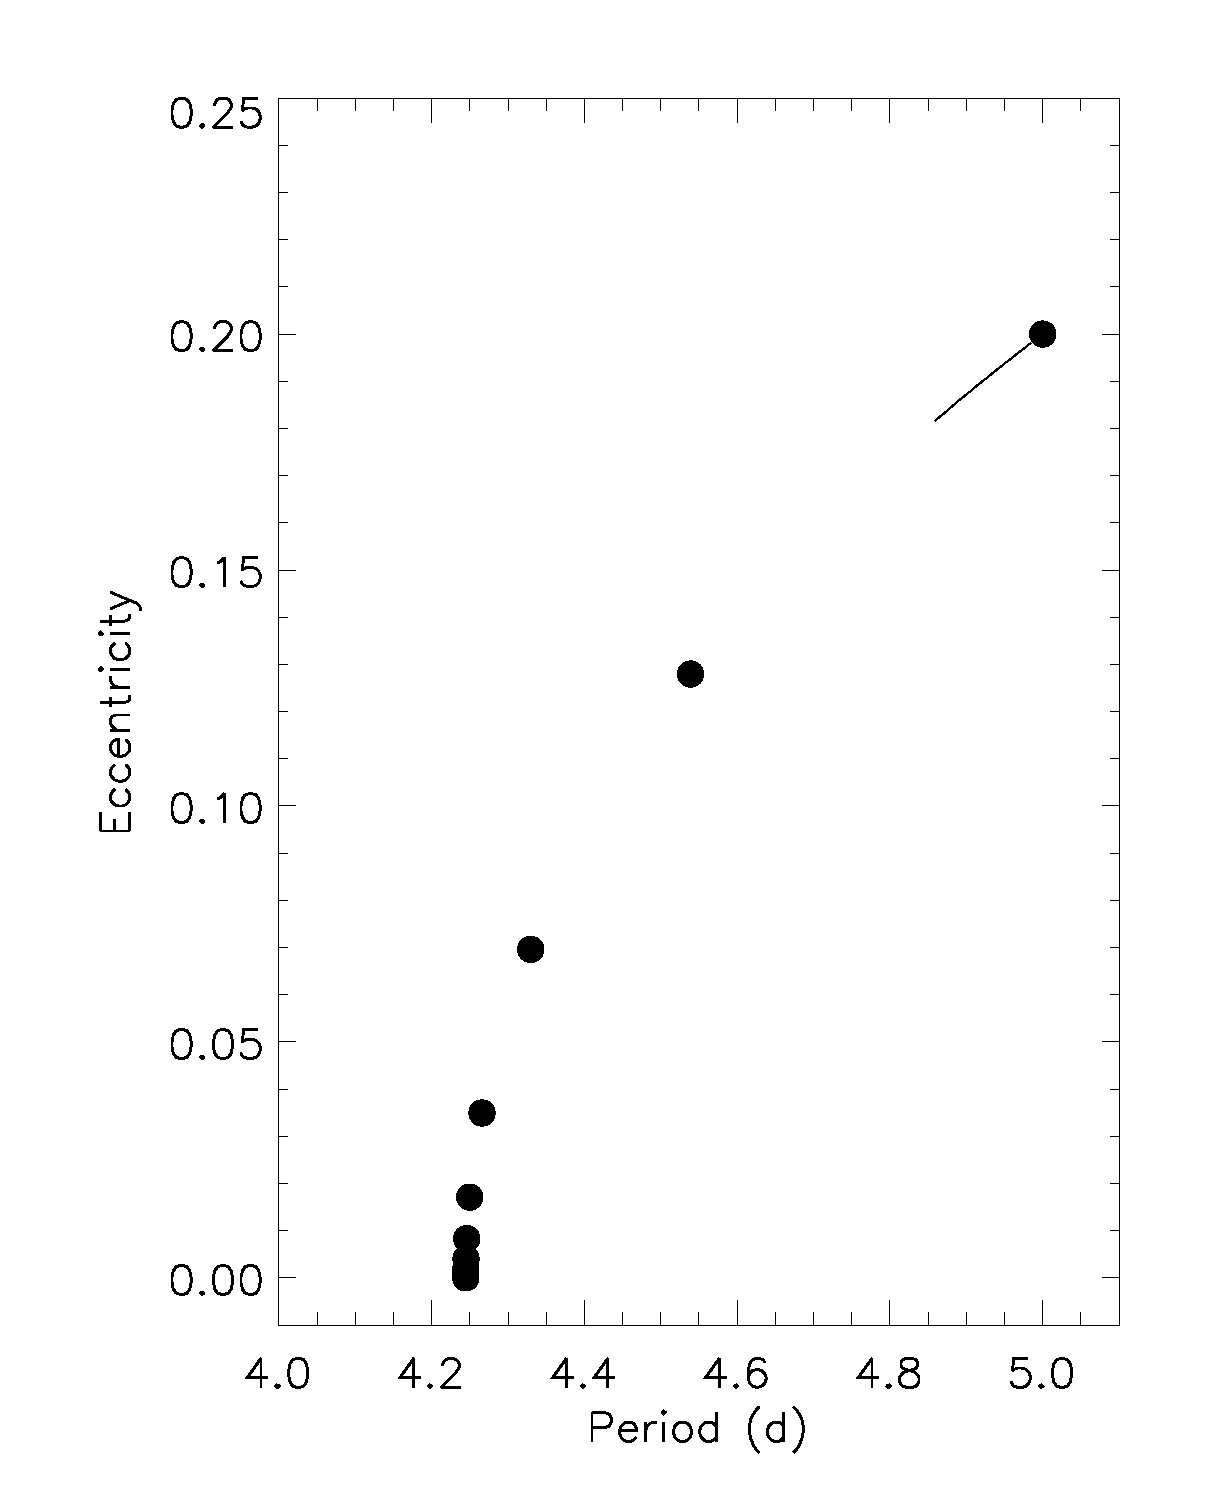
\includegraphics[width=\textwidth]{figures/compq.ps}
  \end{minipage}\hfill
  \begin{minipage}[c]{0.6\textwidth}
    \caption{Comparison of the tidal evolution of a
  2~\rearth~ mini--Neptune (solid line; for 10 Gyr) and a 2~\rearth~
  super--Earth (circles; in 100 Myr intervals).  The mini--Neptune
  experiences little orbital evolution, but the super--Earth
  circularizes in about 1 Gyr.  This discrepancy is due to the 4
  orders of magnitude difference in tidal dissipation between gaseous
  and rocky planets.}
    \label{fig:compareQ}
    \hspace*{\fill}  
    \hrule
  \end{minipage}
\end{figure*}

To test this possibility, we performed the following test. We created
25,000 synthetic star--planet configurations with initial semi--major
axes uniformly in the range [0.01,0.1] AU, radii in the range
[0.5,10]~\rearth, stellar masses in the range [0.8,1.2]~\msun, and
ages in the range [2,8] Gyr.  If the planetary radius is less than 2~\rearth, we
assume Earth-like composition and scale the mass as ($R$/\rearth)$^{3.68}$\mearth~\citep{Sotin07} and
assign a tidal $Q$ in the range [30,300].  If larger than 2~\rearth, then we assume
the density is 1 g/cm$^3$, and a tidal $Q$ in the range
[$10^6$,$10^7$].  The initial eccentricity is drawn from the currently
observed distribution of distant planets ($a > 0.2$~AU)\footnote{www.exoplanets.org}.  We then
integrate the CPL tidal model forward for the randomly chosen age and assume we
observe the system in that final configuration. In
Fig.~\ref{fig:radper}, we show the resulting average eccentricities of
these planets as a function of planetary radius, $R_p$, and orbital
period, $P$.  The small values of $e$ at low $R_p$ and $P$ shows the effect of the large difference in tidal $Q$s.  Furthermore, we can see the features that correspond directly
to three parameters that are currently very poorly constrained:
$R_{crit}$ via the rapid rise in $\avg{e}$ at 2~\rearth; $Q_g$ via the
rapid rise in $\avg{e}$ at 1 day above 2~\rearth; and $Q_r$ via the
rise over 4--8 days and below 2~\rearth.  Thus in this simple model,
we see three constraints for three unknowns, yielding the possibility
that the right observations may provide values for these
elusive quantities.

\begin{figure*}[t] 
  \begin{minipage}[c]{0.39\textwidth}
    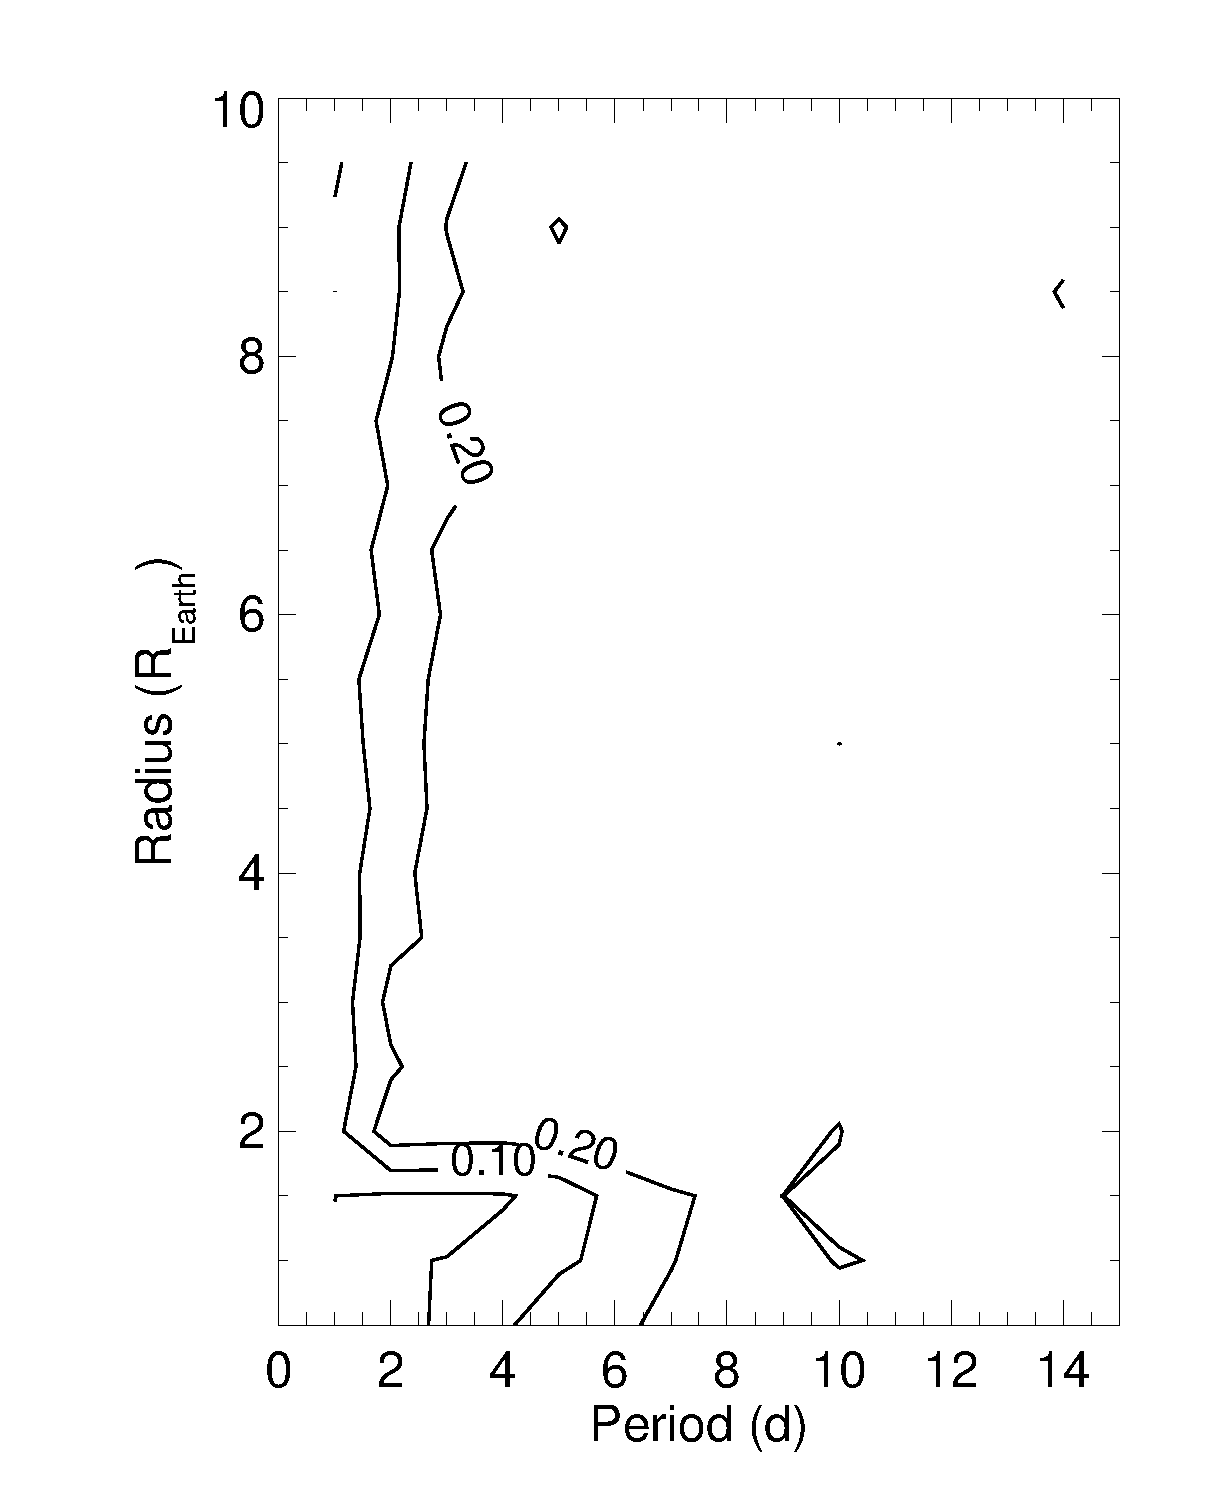
\includegraphics[width=\textwidth]{figures/radper.ps}
  \end{minipage}\hfill
  \begin{minipage}[c]{0.6\textwidth}
    \caption{Average final eccentricity of a suite of 25,000
systems of one star and one planet. Planets larger than 2~\rearth~are gaseous, and 
those smaller are rocky. The binsizes are 0.5~\rearth~ in radius and 0.5 d in period.
Gaseous planets retain a residual eccentricity if $P > 1.5$ d, while rocky planets require
$P > 4$ d. The transition occurs at 2~\rearth, which in this case is $R_{crit}$. }
    \label{fig:radper}
    \hspace*{\fill}  
    \hrule
  \end{minipage}
\end{figure*}


However, as \kepler data do not provide eccentricity, we must transform this output
into a form that is directly comparable to an observable, i.e. $e_{min}$. In order to
calculate $e_{min}$ from these synthetic data, we choose a random
value for $\theta$ and calculate the velocity according to
Eq.~\ref{eq:velocity}. We calculate the average minimum eccentricity
$\avg{e_{min}}$ for our rocky and gaseous planets in 0.5 day orbital
period intervals and plot $\avg{e_{min}}$ as a function of orbital
period for different radii as solid lines in Fig.~\ref{fig:emin}. For
$R < 2$~\rearth, $\avg{e_{min}}
\sim 0$ up to about a 4 day period. However, for larger radii,
circular orbits are only guaranteed for periods less than about 2
days. \textit{Despite the order of magnitude ranges for each physical
  planetary property, the disparity in tidal $Q$'s produces a strong
  signal in $\avg{e_{min}}$ that distinguishes the rocky and gaseous
  planets. }


\begin{figure*}[t] 
  \begin{minipage}[c]{0.39\textwidth}
    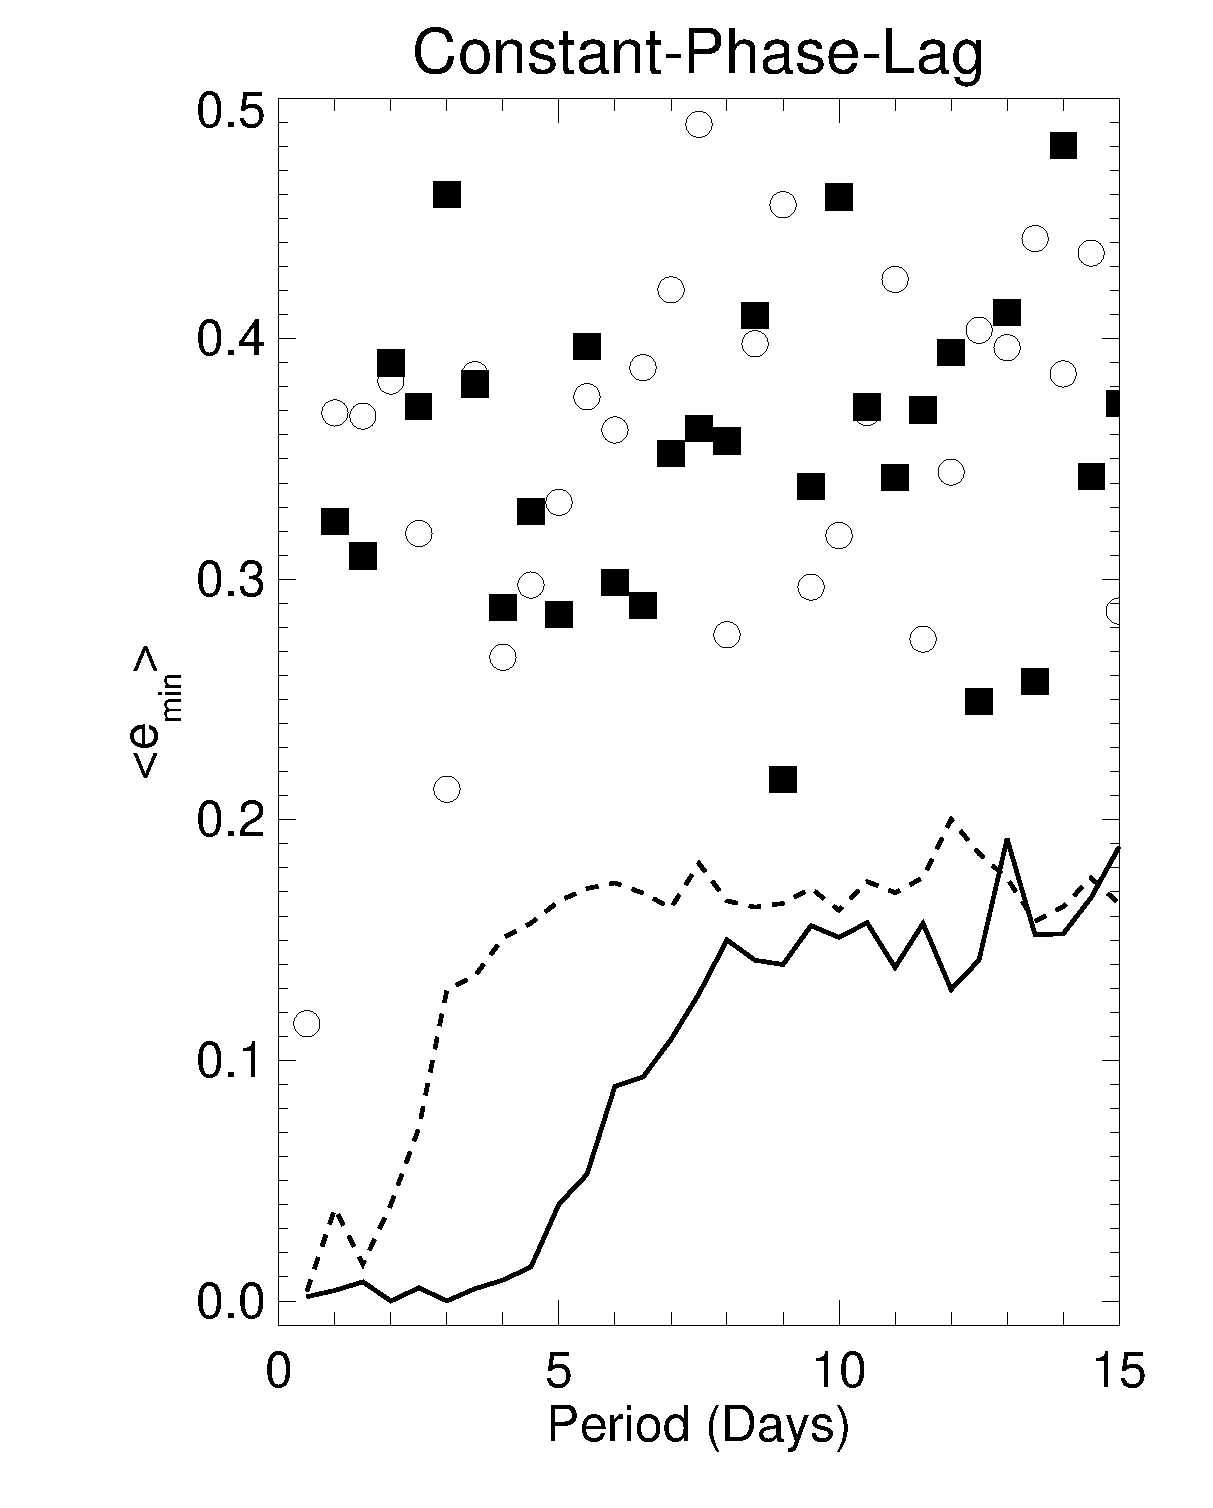
\includegraphics[width=\textwidth]{figures/compare.emin2.ps}
  \end{minipage}\hfill
  \begin{minipage}[c]{0.6\textwidth}

    \caption{Average minimum eccentricities for transiting exoplanets
  as a function of period and radius.  The solid curve and filled
  squares represent planets with radii below the selected critical
  radius of 2~\rearth, while the dashed curve and open circles are
  larger planets. The lines are the relationships for the simulated
  data set, symbols for KOIs. The latter all have values near 0.3--0.4
  days regardless of period, whereas model gaseous planets have
  non--zero eccentricities if the period is larger than 1.5 days, and
  rocky planets at larger than 4. If tidal dissipation is a function
  of exoplanet radius, it should be detectable. }

    \label{fig:emin}
    \hspace*{\fill}  
    \hrule
  \end{minipage}
\end{figure*}

This pilot study is encouraging, but its feasibility rests on the
precision of the models of the \kepler data.  Specifically, impact
parameters, stellar and planetary radii, orbital period, and stellar
mass must be known and their uncertainties well--modeled.  The first
four properties are measurable from transit data alone, while the
fifth must be estimated by other means.  The \kepler team has provided
these data in various publications and websites.  The solid squares
show the values of $\avg{e_{min}}$ with quantities from the
\kepler Planet Candidate Data
Explorer\footnote{http://planetquest.jpl.nasa.gov/kepler}.  Nearly all
the observed data are above the predictions. There are two possible
explanations for this discrepancy: 1) The theory is wrong, or 2) the
reported model parameters are of poor quality.  We outline limits of
the theory next.

\medskip
{\centerline{\ub{\sc Non--Tidal Effects}}}
\smallskip

First, we note that additional companions can pump eccentricity
through mutual gravitational interactions, even if tidal damping is
ongoing \citep{MardlingLin02,Bolmont13}.  Therefore we must be
cautious when interpreting Fig.~\ref{fig:emin}, as additional
companions, both seen and unseen, can maintain non--zero
eccentricities.  However, there are limits: \cite{Bolmont13} showed
that planet--planet interactions cannot maintain the eccentricity of
the hot super-Earth 55 Cnc e above 0.1.  That system is particularly
relevant as there are many close--in planets orbiting a typical G
dwarf.  Therefore, we conclude that eccentricity pumping can be
significant but cannot explain the discrepancy between the observed
and simulated systems shown in Fig.~\ref{fig:emin}.

Another possibility is that stellar winds and activity can strip an
atmosphere, reducing the mass and radius, and potentially changing the
planet from a mini--Neptune to a super--Earth
\citep{Jackson10,Valencia10,Leitzinger11,Poppenhaeger12}.  Recently,
\cite{OwenWu13} argued that the \kepler sample is consistent with
hydrodyanmic mass loss, and that some low--mass planets could have
formed with substantially more mass.  Mass loss should decrease the
time to circularize the orbit, assuming the radius doesn't become very
large, which is unlikely after about 100 Myr \citep{Lopez12}.
Therefore, mass loss could stall circularization for mini--Neptunes,
but not for super--Earths.  Although few radial velocity measurements
exist, planets with radii less than $\sim 1.5$~\rearth~ have densities
consistent with silicate compositions \citep{Batalha11}.  Thus, mass
loss seems unlikely to explain the differences seen for the smallest
candidates in the \kepler field.

Other effects, such as stellar mass loss or the galactic tide will be
negligible, but to properly treat the problem, planetary mass loss and
planet--planet perturbations must be considered.  On the theoretical
side, the path forward to determine $R_{crit}$, $Q_{r}$ and $Q_{g}$ is
clear: We must first model the full range of plausible values for
these three parameters to calculate $\avg{e_{min}}$($R_p,P$); include
the planet--planet interactions of multiple planet systems over the
lifetimes of the systems; and incorporate mass loss, including the
possibility that a mini--Neptune can become a super--Earth with its
associated change in tidal $Q$.

In summary, the effects of tidal circularization appear not to be
present in publicly available fits to the \kepler data, in sharp
contradiction with the radial velocity exoplanet
sample \citep{Butler06}.  These fits are therefore inadequate to
identify $R_{crit}$ and tidal $Q$s, meaning a state--of--the--art
statistical re--analysis of \kepler photometry is required to
determine these fundamental parameters.

\bigskip
\centerline{\bf III. Technical Approach and Methodology}
\addcontentsline{toc}{subsection}{III. Technical Approach and Methodology}
\smallskip

%\medskip
%{\centerline{\ub{\sc Transit Duration}}}
%\smallskip
%
%What is this definition?  Center of planet crossing?
%
%\begin{eqnarray}
%\Delta t_{circ} & = & {{P}\over{\pi}}~{{\sqrt{R_*^2 - b_0^2}}\over{a}} \nonumber \\
%                & = & {{P}\over{\pi}}~{{\sqrt{1 - \beta_0^2}}\over{\alpha}}
%\label{eq-tcirc}
%\end{eqnarray}
%where $P$ is the orbital period in cgs units, $R_*$ the stellar radius
%in cgs, $b_0$ the minimum planetary impact parameter in cgs, $\beta_0$
%a unitless measure of the minimum impact parameter (scaled by the
%stellar radius), $a$ the planetary semi--major axis in cgs, and
%$\alpha$ this value scaled by the stellar radius.

We describe below our technical approach to the re--analysis of Kepler
data, including simulations to understand how we will be able to
constrain system parameters, a validation of this technique using a
known exoplanet system, and outline how we will fold these results
into tidal theory to determine $R_{crit}$, $Q_{r}$ and $Q_{g}$.

We will use the quadratic limb--darkened model
of \cite{2002ApJ...580L.171M} to describe the lightcurves.  We
emphasize that at its core, the Mandel \& Agol model is a purely
geometric one that describes an opaque planetary disk occulting a
limb--darkened stellar disk.  Many applications of this technique use
planetary orbital parameters such as semi--major axis and inclination
as inputs to the model, along with frequent assumptions of zero
eccentricity, {\it but this need not be the case}.  Instead we use a
purely geometric implementation of \cite{2002ApJ...580L.171M} whose
only assumption is that the planet has constant transverse velocity
during transit.  This generalization is especially important for our
proposal, as we need to compare our measured transit duration with
what would be observed in the zero--eccentricity limit.

The main observable in this model is the time it takes the planet to
cross the stellar equator, $\tau$ (this may also be thought of as a
measure of the transverse velocity, $v = R_*/\tau$).  This allows us
to cast $e_{min}$ in terms of $\tau$, period $P$, and the (unknown)
ratio of the planet's semi--major axis to stellar radius.  The
uncertainty in impact parameter will affect our knowledge of the other
system parameters through covariance.  However, this uncertainty may
be marginalized over by examining posterior distributions, which
drives us to use Markov--Chain Monte Carlo (MCMC) modeling in our
analysis, described below.


\medskip
{\centerline{\ub{\sc Transit Model}}}
\smallskip

%To avoid a dependency between the fitted model and a physical model
%that includes orbital dynamics, we parameterize the lightcurve model
%in purely geometric terms.  To do so, w

We adopt the quadratic limb--darkened model
of \cite{2002ApJ...580L.171M}, which describes transit lightcurves in
terms of two (nuisance) limb--darkening coefficients and two
(important) system parameters.  The first of the system parameters is
the planetary radius divided by the stellar radius ($\zeta \equiv
Rp/R_*$), which determines the fractional area of the stellar disk
that may be occulted by the planet.  The second is the instantaneous impact
parameter of the planet ($\beta \equiv b/R_*$).  This variable is a
function of time, due to the objects' relative motion.  This function
is dependent on the chord that the planet takes across the stellar
disk, itself typically estimated using the orbital parameters
semi--major axis ($\alpha \equiv a/R_*$) and inclination.

%\begin{figure*}[t] 
%  \begin{minipage}[c]{0.37\textwidth}
%    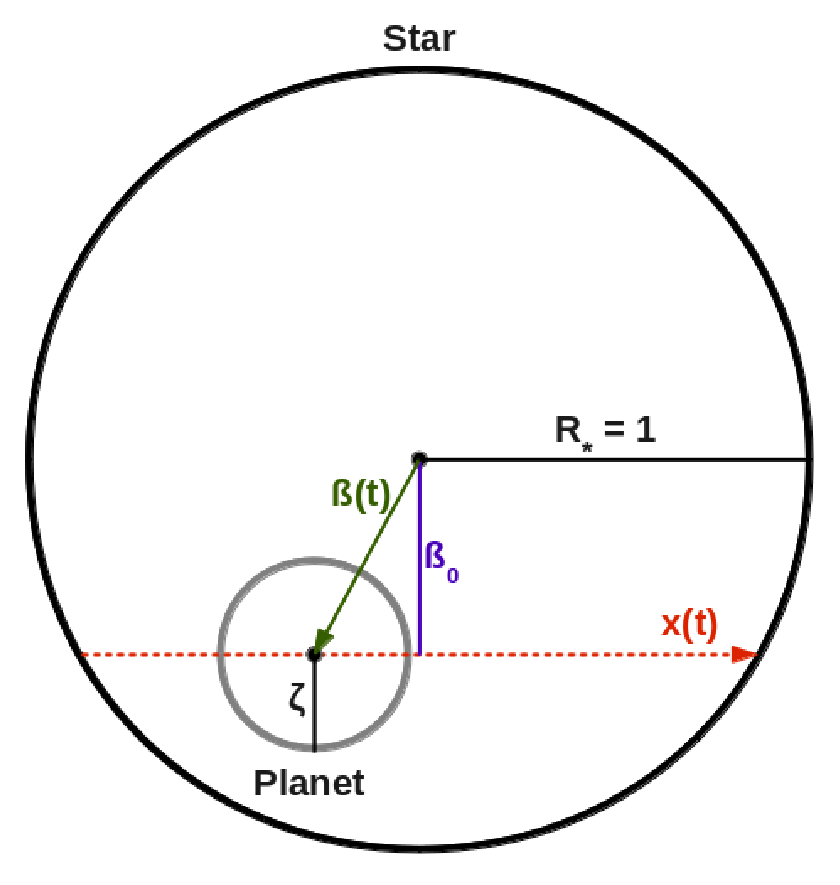
\includegraphics[width=\textwidth]{figures/schem.eps}
%  \end{minipage}\hfill
%  \begin{minipage}[c]{0.6\textwidth}
%    \caption{Schematic detailing our geometric model for the impact
%      parameter as a function of time, $\beta(t)$.  Relevant variables
%      include the minimum impact parameter scaled by the stellar radius
%      $\beta_0$, the radius of the planet scaled by the stellar radius
%      $\zeta$, and the time-dependent position of the planet $x(t)$.  The
%      fitted parameters are $t_0$ (defined where $\beta(t_0) = \beta_0$),
%      the minimum impact parameter $\beta_0$, scaled planetary radius
%      $\zeta$, and $\tau$ (which represents the time for the planet to
%      travel the angular distance subtended by the stellar radius). }
%    \label{fig-schem}
%    \hspace*{\fill}  
%    \hrule
%  \end{minipage}
%\end{figure*}

Instead we describe the impact parameter as a function of time using the
minimum impact parameter $\beta_0$ -- when the centers of the sources
are maximally aligned at center--of--transit time $t_0$ -- and the
location of the planet on the transit chord across the stellar disk.
The coordinate of the planet as a function of time is represented as
$x(t) / R_* = (t - t_0) * v / R_* = (t - t_0) / \tau$, where $v$ is
the (unknown) perpendicular velocity, and $\tau$ is the (fitted)
amount of time it takes the planet to traverse a distance equal to the
stellar radius assuming no acceleration.  This allows us to express
geometrically the impact parameter as a function of time:
\begin{eqnarray}
\beta(t) & = & \sqrt{\beta_0^2 + \left((t - t_0) / \tau\right)^2},
\end{eqnarray}
which is then used along with $\zeta$ to generate a model transit
lightcurve.
This model yields a 4--parameter fit to each transit: $t_0, \beta_0^2,
\tau, \zeta$.  The system period $P$ is determined using 
multiple ($N$) transits and the ensemble of $t_{0;i=1...N}$.  The
transit duration $T$ is found from the 2 solutions to $\beta(t) = 1$:
\begin{eqnarray}
T & = & 2 * \tau \sqrt{1 - \beta_0^2}.
\label{eq-dt}
\end{eqnarray}

Combining Equations~\ref{eq:tdd},\ref{eq:emin} and \ref{eq-dt} we express $e_{min}$ in terms of our model
parameters:
\begin{eqnarray}
e_{min} & = & \left| \frac{P^{2} - 4 \pi^{2} \alpha^{2} \tau^{2}}{P^{2} + 4 \pi^{2} \alpha^{2} \tau^{2}} \right| 
\label{eq-emin2}
\end{eqnarray}
or, more intuitively,
\begin{eqnarray}
e_{min} & = & \left| \frac{1 - (v_c/v)^2}{1 + (v_c/v)^2} \right| .
\label{eq-emin3}
\end{eqnarray}

Equation~\ref{eq-emin2} indicates that $e_{min}$ is purely a function
of the fitted parameter $\tau$, the derived period $P$, and an
externally estimated semi--major axis for the planet (in units of the
stellar radius) $\alpha$.  

%The uncertainty in $e_{min}$ scales as below for all 3 parameters:
%
%\begin{eqnarray}
%\frac{\delta e_{min}}{\delta \xi} & = & \frac{\Xi~e_{min}}{\xi} ~~~~~ \left[\xi = \tau; P; \alpha \right] \\
%{\rm where}~~~~~\Xi & \equiv & \frac{16 \pi^{2} \alpha^{2} \tau^{2} P^{2}}{16 \pi^{4} \alpha^{4} \tau^{4} - P^{4}}.\nonumber
%\label{eq-emin3}
%\end{eqnarray}
%In the limit of a circular orbit ($P \rightarrow 2 \pi \alpha \tau$),
%the product $\Xi~e_{min}$ = 1.

\medskip
{\centerline{\ub{\sc KOI 701.02}}}
\smallskip

We validate our proposed methodology by analyzing \kepler data from KOI
701.02 \citep[Kepler 62--b;][]{2013arXiv1304.7387B}.  This planet has
a period of 5.715 days, $\zeta = 0.018$ (R$_p$ $\sim$ 1.3 R$_E$), and
a transit depth of $4 \times 10^{-4}$.  We use the limb darkening
parameters for the host star from
\cite{2010A&A...510A..21S}.  The \kepler data have correlated (red) noise
which we must account for before model fitting.  To do so, we perform
a local detrending by first dividing the data by the proposed model,
and fitting a low order spline to the result.  The goodness of fit is
determined by comparing the product of the spline and the model to the
data.  We were able to model the first 32 transits before this
proposal deadline.

%Figure~\ref{fig-koi70101} provides an example model fit determined in
%this manner.  The data used are the {\tt PDCSAP} fluxes and
%uncertainties.  

%\begin{figure*}[t] 
%  \begin{minipage}[c]{0.6\textwidth}
%    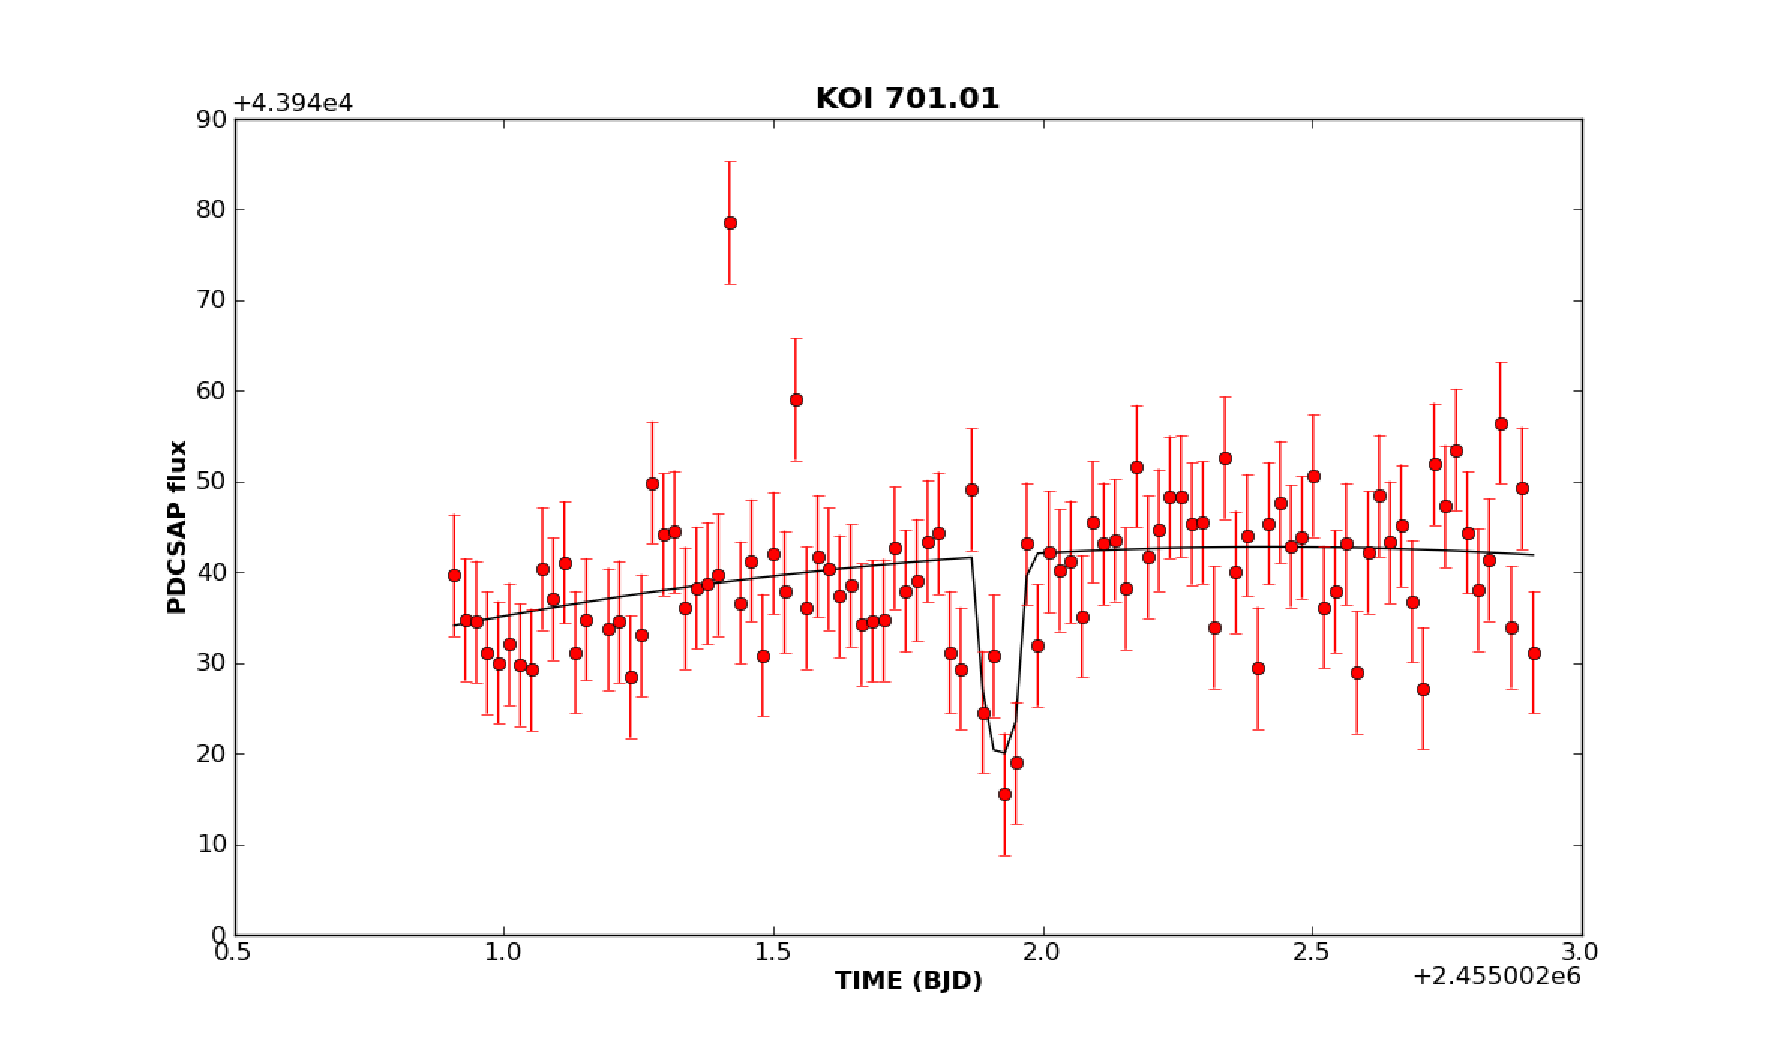
\includegraphics[width=\textwidth]{figures/701.01.eps}
%  \end{minipage}\hfill
%  \begin{minipage}[c]{0.4\textwidth}
%    \caption{An example of our local detrending algorithm, applied to
%      the first transit of KOI 701.02.  The data and model (solid
%      line) are in {\tt PDCSAP} flux units.  The solid curve is
%      generated by first dividing the data by the transit model,
%      applying a low--order spline to the normalized data, and then
%      taking the product of the spline and the model.}
%    \label{fig-koi70101}
%    \hspace*{\fill}  
%    \hrule
%  \end{minipage}
%\end{figure*}

To examine how our knowledge of system parameters evolves as a
function of number of transits, we have fit {\it all} the data up to
the time of each transit, for each of $N = 32$ transits.  This means
that for transit $n \leq N$, we have common model parameters
$\beta_{0}^2, \tau, \zeta$ and per--transit parameters $t_{0;i=1..n}$,
for a total of $n+3$ model parameters.  This yields an ensemble of $N$
system models, each incorporating one more transit than the previous
one.

We used the affine--invariant MCMC sampler {\tt emcee}
\citep{2013PASP..125..306F} to sample the posterior distribution of
the model parameters.  This program uses the method of
\cite{Goodman-Weare} to achieve high sampling performance independent
of the aspect ratio of the posterior distribution, meaning covariances
between parameters are less important to the efficacy of the MCMC
sampling.  This provided a set of MCMC chains that we examine to
determine our constraints on the fitted parameters.  We used the
Gelman--Rubin $\hat{\rm R}$--statistic \citep{Gelman92} to assure that
each chain sufficiently samples model space, and required effective
chain lengths larger than $10^4$ to ensure sufficient mixing in the
MCMC sample \cite[e.g.][]{2004PhRvD..69j3501T}.  Our trial runs using
KOI 701.02 indicated that our chains typically have autocorrelation
lengths of $\sim 100$, requiring a total number of steps per chain of
$10^6$.  We used burn--in times having 10\% the requested number of
steps, which are then discarded before the final chain commences.

%For each transit, we evaluated the joint and marginalized
%distributions of fitted parameters $\zeta$ and $\tau$.
%
%Figure~\ref{fig-joint} demonstrates how the joint distribution evolves
%from fitting 1 transit (dashed contours, which represent 68.3\%,
%95.5\%, and 99.7\% confidence limits), to fitting 32 transits (solid
%contours, at the same confidence limits), for KOI 701.02.
%
%We then marginalized over all other parameters, to examine the
For each transit, we marginalized over all other parameters, to
examine the per--parameter confidence limits.  Figure~\ref{fig-marg}
demonstrates how our marginalized constraints on $\tau$ (left panel)
and $\zeta$ (center panel) evolved as a function of the number of
transits used in the fit for 701.02.  The solid line provides the
maximum of the posterior distribution, and the dashed line indicates
its median.  The shaded area encloses 68.3\% of the distribution.  In
this manner, we find a maximum likelihood value of $\tau =
0.051_{0.002}^{0.003}$.  This may be contrasted to $\tau = 0.049 \pm
0.003 $ derived from reported \cite{2013arXiv1304.7387B} parameters,
where they used 171 transits.  For completeness, we note our
confidence limits on $\zeta = 0.0182_{0.0003}^{0.0006}$ vs
the \cite{2013arXiv1304.7387B} result $\zeta = 0.0188 \pm 0.0003$.

% tau 32 0.0508 - 0.0023 + 0.0026
% zeta 32 0.01821 - 0.00029 + 0.0006

%\begin{figure*}[t] 
%  \begin{minipage}[c]{0.47\textwidth}
%    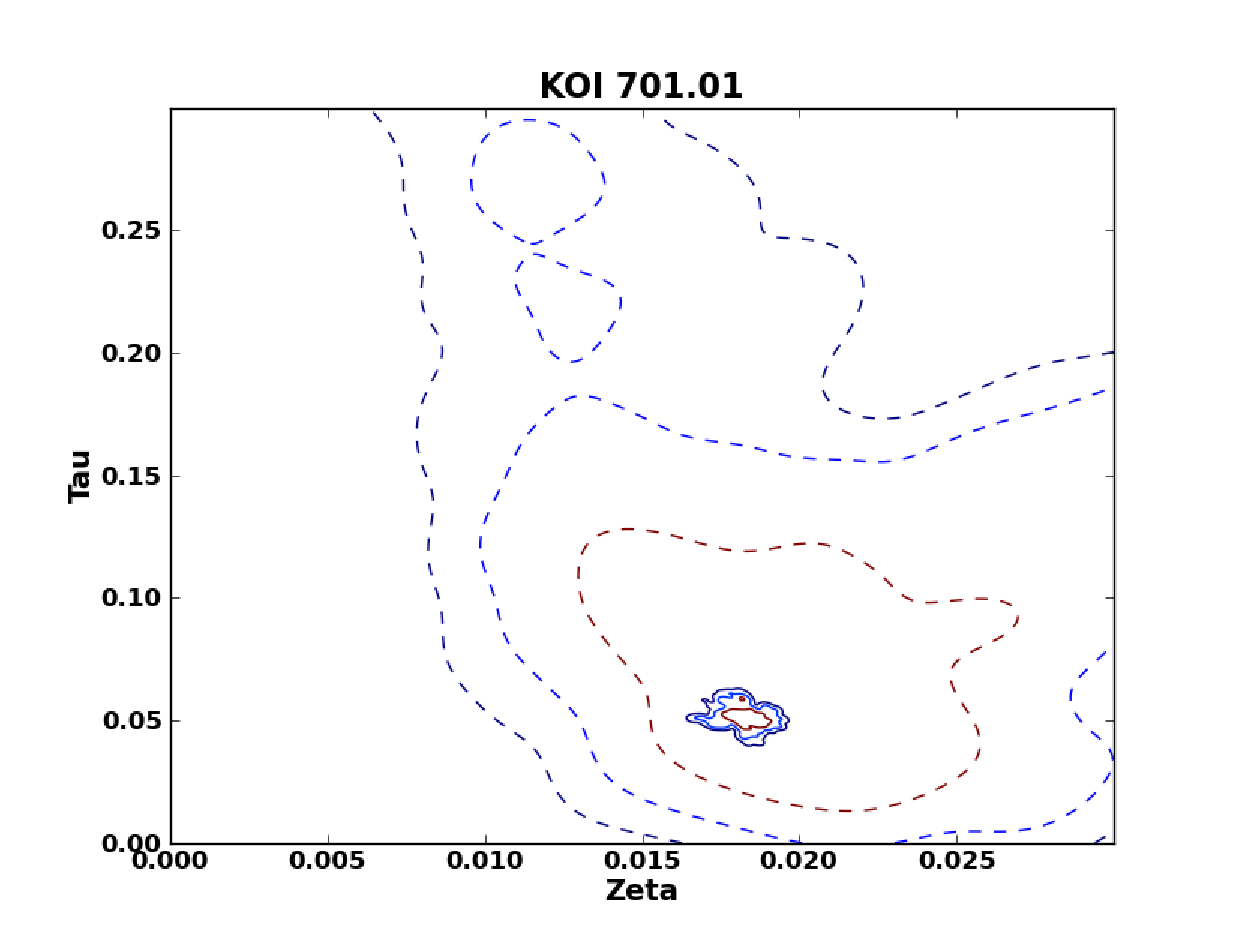
\includegraphics[width=\textwidth]{figures/joint.eps}
%  \end{minipage}\hfill
%  \begin{minipage}[c]{0.5\textwidth}
%    \caption{The joint distribution of $\tau$ vs. $\zeta$ for KOI
%      701.02.  The {\it dashed} lines show the distribution when
%      fitting 1 transit, with contours at the 68.3\%, 95.5\%, and
%      99.7\% confidence limits.  The {\it solid} lines show the
%      distribution when fitting 32 transits simultaneously.}
%    \label{fig-joint}
%    \hspace*{\fill}  
%    \hrule
%  \end{minipage}
%\end{figure*}


\begin{figure*}[t] 
\begin{center} 
\mbox{
\subfigure{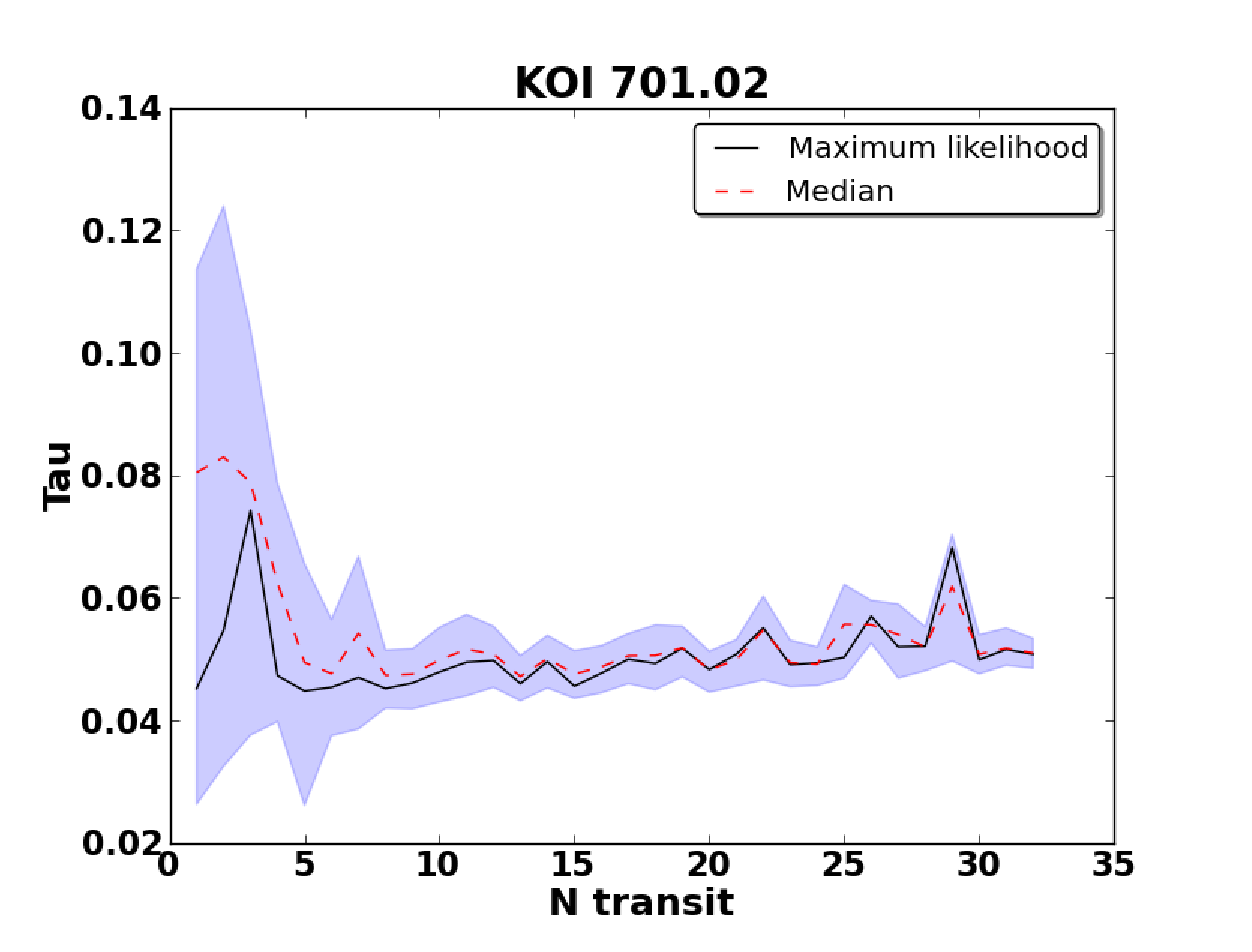
\includegraphics[width=0.31\textwidth]{figures/tau.eps}}
\quad
\subfigure{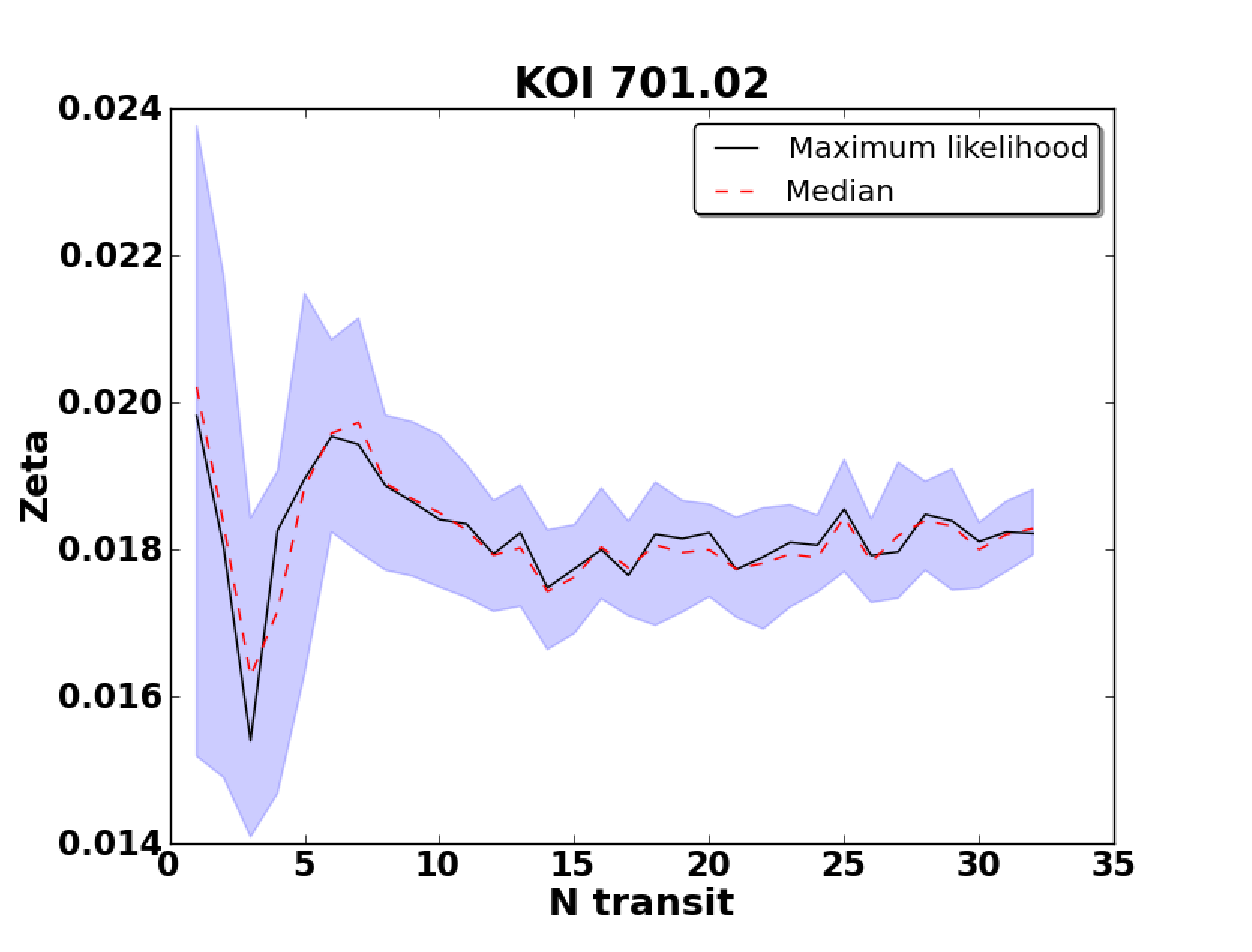
\includegraphics[width=0.31\textwidth]{figures/zeta.eps}}
\quad
\subfigure{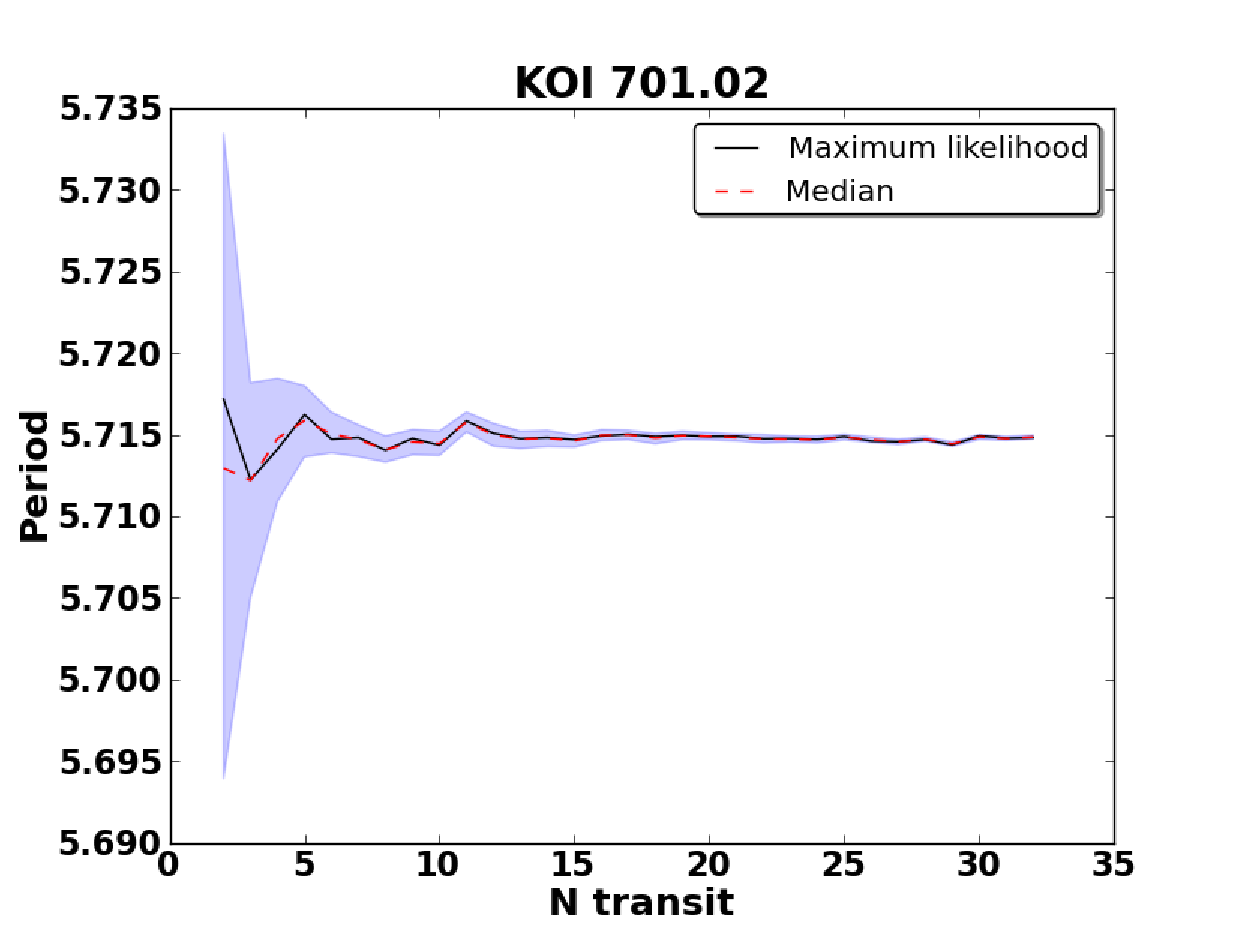
\includegraphics[width=0.31\textwidth]{figures/period.eps}}
}
\caption{The marginalized distributions of $\tau$ (left panel),
  $\zeta$ (center panel), and period $P$ (right panel) as a function
  of the number of transits being used, for KOI 701.02.  For each
  transit $n \leq 32$ we use {\it all} data up to and including
  transit $n$.  The {\it solid} line
  represents the maximum of the posterior distribution, while the {\it
  dashed} line indicates its median.  The shaded area contains 68.3\%
  of the posterior samples.}
\hspace*{\fill}  
\hrule
\label{fig-marg} 
\end{center} 
\end{figure*}

To examine our constraints on the system period, we used the
$t_{0;1..n}$ posterior distributions from the fits described above.
We used {\tt emcee} to sample the posterior space of (nuisance
parameter) $t_{0;1}$ and period $P$.  For a given trial ($t_{0;1}, P$)
pair, the likelihood was determined through:
\begin{eqnarray}
\mathcal{L}(t_{0;1}, P) & = & \prod_{i=1}^{i=n} \kappa_i(t_{0;1} + P * (i-1))
\end{eqnarray}
where $\kappa_i$ is a kernel density estimate of each posterior
distribution $t_{0;i}$, which is evaluated at the predicted time of
transit $t_0 + P * (i-1)$.  By modeling the times of transit
separately in the original MCMC analysis, we allow the possibility of
using a more complex ephemeris model at this stage of the analysis,
such as may be expected from transit timing variations
\citep{2005MNRAS.359..567A,2005Sci...307.1288H}.  The results of this
analysis for KOI 701.02 are presented in the right panel of
Figure~\ref{fig-marg}.

For the derived period after 32 transits, we find $P =
5.71484_{0.00015}^{0.00009}$.  The uncertainty in the period roughly
scales as a power law with an e--folding timescale of approximately 15
transits.  This may be contrasted to $P = 5.714932 \pm 0.000009$ days
reported in \cite{2013arXiv1304.7387B}.  The differences in $e_{min}$
are more substantial.  Using their reported value of $\alpha =
18.7 \pm 0.5$, we derive $e_{min} = 0.043 \pm 0.009$, compared to
$e_{min} = 0.021 \pm 0.005$ using the \cite{2013arXiv1304.7387B}
results.  This difference is almost entirely driven by the (1--sigma)
differences in $\tau$, which makes it of utmost importance to model
this parameter directly.

To examine our ability to constrain system parameters as a function of
transit depth and signal--to--noise (S/N), we generated simulated
lightcurves at the \kepler cadence.  We used a subset of the synthetic
systems described in the first section of this proposal.  For each, we
simulated lightcurves at magnitude 8/10/12/14, adding a random draw
from a Gaussian with widths 11.3/29/80/296 ppm (respectively) to each
datapoint to simulate white noise.  We find that after 10 transits, we
are able to recover $\tau$ to better than ten percent for all transits
deeper than 0.5\% down to 14$^{th}$ magnitude; deeper than 0.1\% down
to 12$^{th}$ mag; deeper than 0.05\% down to 10$^{th}$ mag; and deeper
than 0.01\% down to 8$^{th}$ mag.  This analysis is consistent with
our results from KOI 701.02, where the host star's magnitude is 13.6,
the transit depth is 0.04\%, and measured S/N in $\tau$ is $\sim$ 7.8
after modeling 10 transits: $0.0479_{0.0049}^{0.0073}$.  Note the
measured precision in $\tau$ increases to a S/N of approximately 20
after 32 transits (Figure~\ref{fig-marg}).

%\begin{figure*}[t] 
%  \begin{minipage}[c]{0.57\textwidth}
%    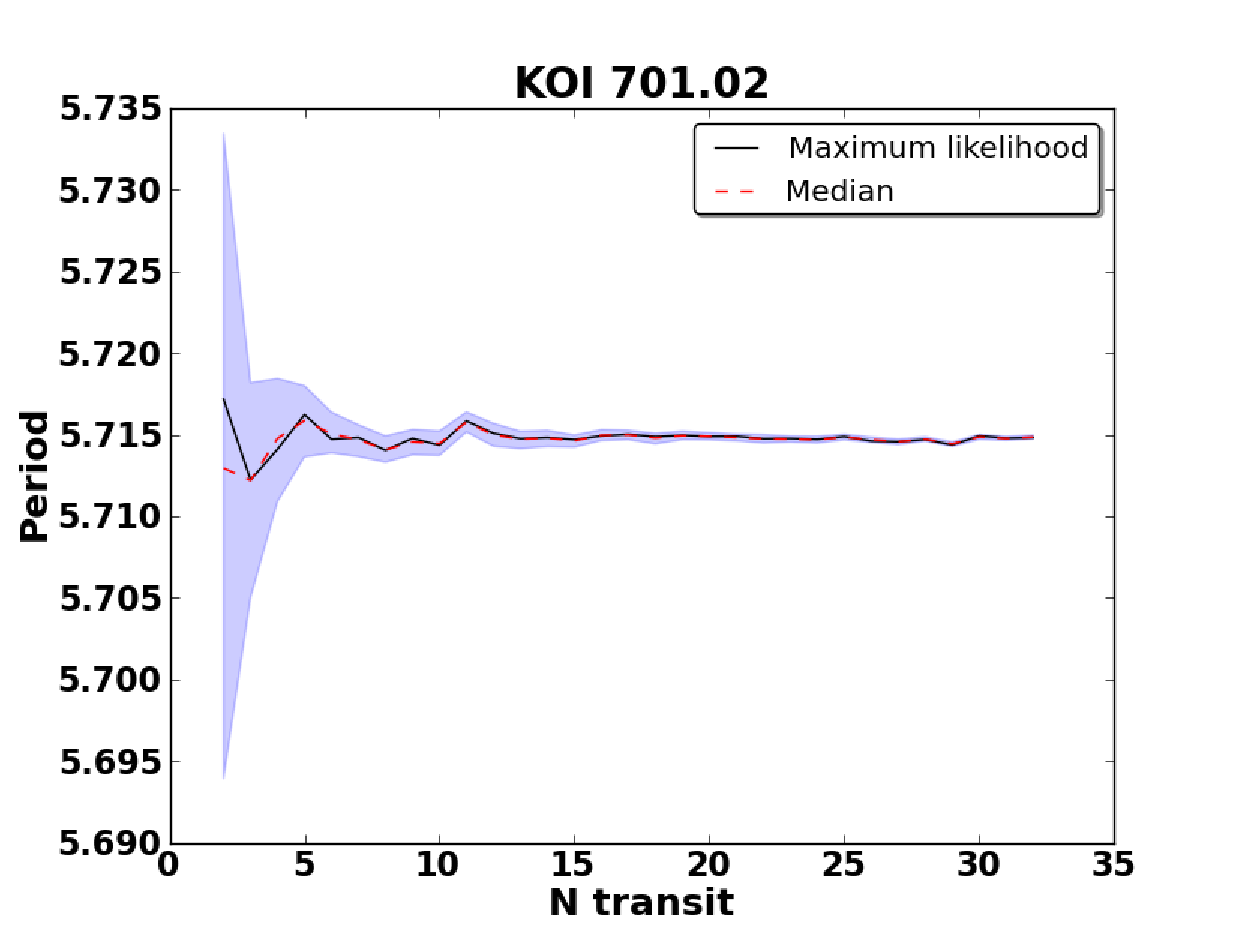
\includegraphics[width=\textwidth]{figures/period.eps}
%  \end{minipage}\hfill
%  \begin{minipage}[c]{0.4\textwidth}
%    \caption{The evolution of the posterior distribution on orbital
%      period $P$ (y--axis) based upon the results of modeling $n$
%      times--of--transit (x--axis) separately.  The period posterior
%      is generated by taking the product of the time--of--transit
%      posteriors ($t_{0;i=1..n}$) evaluated at the predicted transit
%      times.  }
%    \label{fig-period}
%    \hspace*{\fill}  
%    \hrule
%  \end{minipage}
%\end{figure*}

%\medskip
%{\centerline{\ub{\sc Lightcurve Simulations}}}
%\smallskip

%To examine our ability to constrain system parameters (in
%particular, $\tau$) as a function of transit depth and
%signal--to--noise (S/N), we generated simulated lightcurves at
%the \kepler cadence.  We used a subset of 6 of the synthetic systems
%described in the first section of this proposal.  These were chosen to
%have transit depths of [5e-5/1e-4/5e-4/1e-3/5e-3/1e-2] percent.  We
%use the system inclination, semi--major axis, planet--to--star radius
%ratio, and period (along with two limb darkening parameters) to
%generate fake system lightcurves using the method of
%\cite{2002ApJ...580L.171M}.  The system lightcurve is evaluated once
%each minute and integrated over 30 evaluations to approximate a single
%\kepler long--cadence observation.  This is done for a window of 1 day
%on either side of the given transit midpoint to ensure significant
%out--of--transit data to include in the fit.

%A white--noise component is added to each lightcurve for each of 4
%magnitude bins, using the precisions in parts--per--million (ppm)
%given on the \kepler calibration
%webpage \footnote{http://keplergo.arc.nasa.gov/CalibrationSN.shtml}.
%We evaluate each lightcurve separately for magnitude 8/10/12/14
%objects, adding a random draw from a Gaussian with widths
%11.3/29/80/296 ppm (respectively) to each datapoint as generated
%above.  We do not include red noise, or other transient gaps and
%features known to exist in the \kepler data.  We then model these data
%using our geometric parameterization.  Figure~\ref{fig-dtau} outlines
%how our signal--to--noise on $\tau$ scales with the system brightness
%and transit depth {\it after fitting 10 transits only} (due to
%computational constraints).  We are able to recover $\tau$ to better
%than ten percent for all transits deeper than 0.5\% down to 14$^{th}$
%magnitude; deeper than 0.1\% down to 12$^{th}$ mag; deeper than 0.05\%
%down to 10$^{th}$ mag; and deeper than 0.01\% down to 8$^{th}$ mag.
%This analysis is consistent with our results from KOI 701.02, where
%the host star's magnitude is 13.6, the transit depth is 0.04\%, and
%measured S/N in $\tau$ is $\sim$ 7.8 after modeling 10 transits:
%$0.0479_{0.0049}^{0.0073}$.  Figure~\ref{fig-dtau} predicts a S/N of
%5--6.  Note the measured precision in $\tau$ increases to a S/N of
%approximately 20 after 32 transits (Figure~\ref{fig-marg}).

%\begin{figure*}[t] 
%  \begin{minipage}[c]{0.47\textwidth}
%    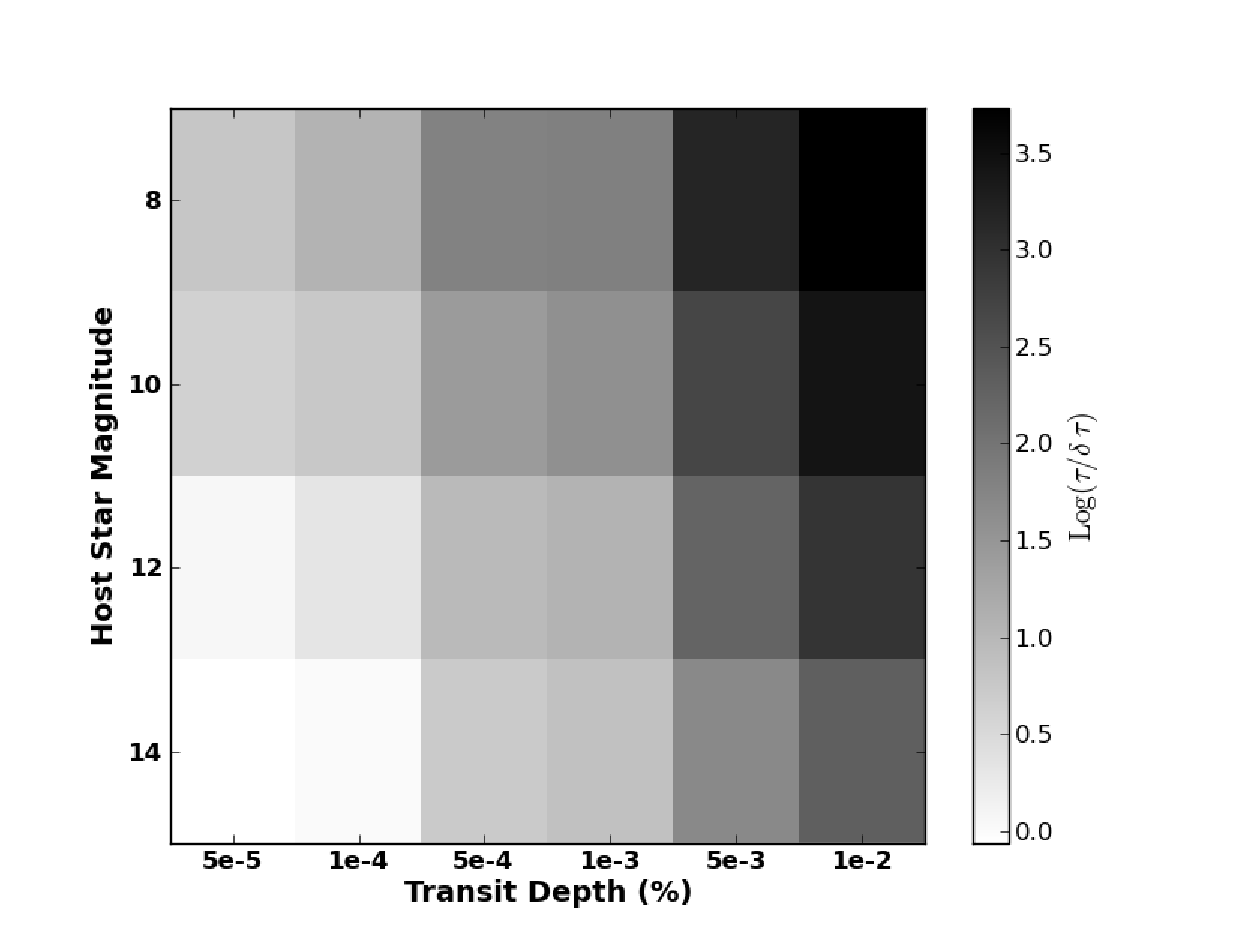
\includegraphics[width=\textwidth]{figures/delta_tau.eps}
%  \end{minipage}\hfill
%  \begin{minipage}[c]{0.5\textwidth}
%    \caption{Grid of signal--to--noise in $\tau$ as a function of host
%    star brightness and transit depth, derived from fitting our
%    geometric model to simulated noisy lightcurves.  The host star
%    brightness sets the S/N of the photometry.  These
%    values were obtained after modeling 10 transits jointly.  These
%    simulations accurately predict the S/N of $\tau$ measurements in
%    KOI 701.02 after 10 transits.}
%    \label{fig-dtau}
%    \hspace*{\fill}  
%    \hrule
%  \end{minipage}
%\end{figure*}

%[[ 0.79372962  1.07761448  1.79022733  1.82613462  3.16994564  3.73020785]
% [ 0.62639459  0.76120963  1.43324592  1.59635851  2.69282439  3.42917786]
% [ 0.06015757  0.32601639  0.96253504  1.07046032  2.24052672  2.9520566 ]
% [-0.06110349  0.0199895   0.73047463  0.86371544  1.69282439  2.3152345 ]]
%[[  6.21912976e+00   1.19567868e+01   6.16917835e+01   6.70092293e+01    1.47892328e+03   5.37288880e+03]
% [  4.23052819e+00   5.77044927e+00   2.71172675e+01   3.94783056e+01    4.92974425e+02   2.68644440e+03]
% [  1.14857027e+00   2.11844107e+00   9.17349940e+00   1.17614352e+01    1.73990974e+02   8.95481466e+02]
% [  8.68753383e-01   1.04710322e+00   5.37619028e+00   7.30660176e+00    4.92974425e+01   2.06649569e+02]]

\medskip
{\centerline{\ub{\sc Target Selection and Characterization}}}
\smallskip

We have examined the current KOIs to establish a preliminary target
list.  We find 1168 objects with appropriate values of $P$ and $R_p$,
and with host star mass estimates between 0.7 and 1.4 \msun, i.e. FGK
stars.  We expect this list to expand somewhat with on--going study of
the \kepler data; we anticipate running our pipeline on approximately
1300 systems.

As described above, our analysis requires a measure of the orbital
separation relative to the stellar radius, $\alpha = a / R_*$, to
derive $e_{min}$ (Equation~\ref{eq-emin2}).  The separation is
obtained trivially from Kepler's 3rd Law according to, $a = (M_*
P^{2})^{2/3}$ where $M_*$ is the mass of the host star.
Unfortunately, the mass of an isolated star is not directly
observable.  Instead, it must be inferred by comparing observed
stellar properties to theoretical stellar evolution models and/or
empirical calibrations.  Thus, to derive the stellar mass, we will
interpolate state-of-the-art stellar evolution models from the
Dartmouth group \citep{Dotter2008} in three parameters: effective
temperature ($T_{eff}$), metallicity ([Fe/H]), and gravity ($log~g$),
as we (L.~Hebb) have done for many other confirmed transiting planets
with radial velocity measurements \citep[e.g.][]{Hebb2009,Hebb2010}.

%Although the stellar parameters are available for all the KOI objects
%in the Kepler Input Catalogue, these values are based on broad band
%colors and are known to have systematic
%problems \citep{Muirhead2012,Pinsonneault2012}.  Therefore, we will
%derive the host star mass using the $T_{eff}$ and [Fe/H] derived
%directly from spectra through stellar characterization techniques.
%While $T_{eff}$ and [Fe/H] can be determined with high precision from
%the stellar spectrum, $log~g$ is usually poorly constrained, and thus
%stellar masses derived from the spectroscopic $log~g$ can have large
%uncertainties and can suffer from systematics.

We plan to primarily use the information available in the literature
for $T_{eff}$ and [Fe/H].  Several teams have large, observing programs
to obtain spectra of KOIs.  \citet{Everett2013} derived stellar
parameters for $\sim 400$ faint KOIs from low resolution data;
approximately 1000 targets have been observed with Keck HIRES
(J.~Johnson et al.\ in prep) and are currently being analyzed with a
new Spectroscopy Made Easy (SME) pipeline (Cargile, Hebb et al.\ in
prep); and the 2.5m Nordic Optical Telescope (NOT) has an ongoing
program to derive stellar parameters of Kepler KOIs (L. Buchave, PI).
However, if certain targets lack observed spectra or derived stellar
parameters, we will obtain the necessary data with the ARC 3.5m
echelle spectrograph through the University of Washington's guaranteed
access to the Apache Point Telescopes.  We will analyze these data as
necessary with our SME pipeline, as we have done for many other
targets \citep[e.g.][]{Wisniewski2012}.

We will obtain the $log~g$ values based on a novel characterization of
the high frequency variability in the {\it Kepler} light curves
(Bastien, Stassun et al.\ 2013, to appear in Nature) which has been
shown to reproduce the exquisite astroseismically measured $log~g$
values \citep{Huber2013} for dwarf and subgiant stars.  The authors
present a technique that can be used to derive $log~g$ values for the
majority of Kepler targets with uncertainties of $\le 0.1$ by
empirically detecting granulation on the stellar surface.  This allows
for significantly more accurate and precise gravity measurements than
can be derived from typical modeling of broad absorption line wings.

We will interpolate the Dartmouth models considering the uncertainties
in the photometrically measured $log~g$ and in the spectroscopically
determined [Fe/H] and $T_{eff}$.  Typical uncertainties of $\le
0.1$~dex in [Fe/H], $\le 100$~K in $T_{eff}$, and $\le 0.1$ in $log~g$
result in uncertainties on the resulting stellar mass of $5-8$\% for
well understood F, G and K-dwarf stars.  This error budget includes
the formal errors from the measured uncertainties on the parameters,
and systematic uncertainties arising from variation between different
stellar evolution models
\citep[2-4\%;][]{Southworth2009}.  We expect to generate a
catalogue of $\alpha = a/R_*$ values for all the short period KOI
transiting planet candidates in our sample with conservative
uncertainties of $\le 10$\%.  Finally, our comparison of the stellar
parameters to the evolutionary models also allows us to estimate
stellar age, which is critical to understanding the tidal quality
factors.

\medskip
{\centerline{\ub{\sc Computational Requirements}}}
\smallskip

%Using KOI 701.02 as a benchmark, we find a roughly quadratic
%relationship for the total {\tt emcee} computation time vs the number
%of transits: $time(n) = -12.5 + 32.2 \times n + 11.9 \times n^2$
%seconds (on a single 2.13 GHz core).  This relationship was
%established using a fixed number of 100 burn--in and 1000 ``final''
%steps for each of $2 \times n + 6$ walkers (i.e. 2 walkers for each
%parameter in the model).  If we scale these chains up to $10^6$ total
%steps, which should yield effective chain lengths of $\sim 10^4$, we
%find a linear relationship in the computation time required to reach
%$10^6$ steps: $time_{10^6}(n) = -1105 + 5943 \times n$ seconds.  

Using KOI 701.02 as a benchmark, we find a linear relationship in the
computation time required to reach $10^6$ steps vs. the number of
transits: $time_{10^6}(n) = -1105 + 5943 \times n$ seconds.
%
For a 5--day period system having $\sim$ 300 transits over the assumed
17--quarter operational lifetime of \kepler, this comes out to $\sim$
21 CPU--days of analysis.  The {\tt emcee} code is natively able to
use multiprocessing capabilities, making this trivial to implement on
a multi--core system.  However, with $\sim 1300$ systems on our
analysis path, this will require $\sim 75$ CPU--years of computation,
requiring the use of NASA's High-End Computing (HEC) facilities.  We
will also make use of the local {\tt Hyak} compute cluster when it is
available.

\medskip
{\centerline{\ub{\sc Data Interpretation}}}
\smallskip

In the following sections, we describe the theoretical component of
our research plan in more detail.  In Task A, we consider systems
consisting of one star and one planet.  In Task B, we include multiple
planet systems. In Task C, we incorporate mass loss.  For each task,
our final step will be a comparison between simulated data and the
ensemble of well--characterized \kepler targets.  This will be done by
comparing the measured distributions of $e_{min}$ to those simulated
using $R_{crit}$, $Q_r$, and $Q_g$ (and possibly factoring in
multiplicity, metallicity, and mass loss).

\medskip
{\centerline{\ub{\sc Task A: Tides in Star--Planet Systems}}}
\smallskip

We begin with the simplest treatment, a single planet orbiting a
single star in an orbit that can be modified by tides.  We will mostly
follow the procedure described for our pilot study, but will expand
the analysis to a broader range of initial conditions as well as
include alternative tidal models.  The pilot study (25,000 simulations
of $\sim 5$ Gyr each) required about 4 hours on a modern workstation,
and therefore many such trials are easily tractable.  The free parameters are the mass--radius
relationship for both rocky and gaseous bodies, the value of
$R_{crit}$, the $Q$s of rocky and gaseous bodies, the initial
eccentricity distribution, and the age distribution of \kepler stars.

The choices in the pilot study were necessarily limited, and we will
explore many more options during this investigation.  While we assumed that
rocky bodies were Earth--like in their composition, other scaling laws
are possible \citep[e.g.][]{Seager07,Fortney07,Lissauer11}.  We will
use these other scalings for the masses of the rocky planets, as well
as mixing the models to allow for a range of compositions.  For the
gaseous planets, we will assume different densities in the range 0.5
-- 3 g/cm$^3$.  The value of $R_{crit}$ is the parameter we are most
interested in; we will grid from 1 to 2.5
\rearth in 0.1~\rearth intervals.  We will consider two different
models for $Q$($R$), the tidal $Q$ as a function of planetary radius.
First we will use the same differences as in the pilot study, but we
will also consider a three--tiered model, in which intermediate mass
planets have intermediate $Q$s.  Neptune, and possible even Saturn,
have a $Q$ value of $10^4$ \citep{ZhangHamilton08,Lainey12}, and hence
we must consider this possibility.  This also introduces a new
radius cut--off, $R_{mid}$, which we will allow to move from 2 to
5~\rearth.  The $Q$ range for these systems will have values between
3000 and 30,000.  We will randomly choose a stellar mass in the range
0.7--1.4~\msun as we are interested in FGK stars.  Finally, we will
keep the initial eccentricity distribution consistent with that of
more distant exoplanets.  Ultimately we expect to run several hundred
suites of systems, easily do--able on a modern multi--core
workstation.

The examples in Figs.~\ref{fig:compareQ}--\ref{fig:emin} used one
tidal model, in which the lag angle between the tidal bulge and the
perturber is constant regardless of frequency
\citep[e.g.][]{GoldreichSoter66,Jackson08}.  Another popular model
assumes that the lag angle is instead a function of frequency
\citep[e.g.][]{Hut81,Matsumura10}.  We will also employ this model
with the same ranges as described above, and relating $Q$ to the time
lag $\tau$ as $Q = 1/n\tau$, where $n$ is the mean motion
\citep[e.g.][]{Correia12}.  In reality there is no general conversion between
the two, but this relation is in common use.  Thus, our work may also
shed light on the frustrating ambiguity in determining the most
appropriate equilibrium tidal model.

\medskip
{\centerline{\ub{\sc Task B: Multi--planet Systems}}}
\smallskip

Mutual
gravitational interactions between planets can maintain an
eccentricity, even in the presence of strong tidal damping
\citep{MardlingLin02,GreenbergVanLaerhoven11,Correia12}.  To assess this effect, we
will perform simulations of multiplanet systems undergoing tidal
damping. The Gyr 
timescales for damping are too long for accurate N-body modeling, so will use classical secular theory to model the planet-planet interactions. The second order theory is
insufficient for many of the cases we consider, which will have
eccentricities up to 0.9.  Therefore, we will use higher order
theories, which have been previously developed
\citep[e.g.][]{Ford00,VerasArmitage04,LibertHenrard05}. To maximize accuracy, and take advantage of the high degree of coplanarity of close--in
\kepler systems \cite{Fabrycky12}, we will use the coplanar 12th order theory of \cite{LibertHenrard05} to evaluate
the evolution.

More challenging is the choice of initial conditions.  While many
\kepler systems are multiple, we do not yet know the underlying
distribution of orbital architectures.  A full exploration of
parameter space with arbitrary multiplicity and orbital elements would
be intractable.  We
therefore will limit our study to suites of 25,000 systems with
multiplicity that follows from the observations.  To better match
the \kepler systems, we will limit the size of our planetary systems
to $<0.5$ AU. The physical properties of the planets will be in the
same ranges as above. We will perform numerical tests of stability of
initial conditions, and will throw out systems that divergently cross
strong mean motion resonances -- such 2:1, 3:1, and 3:2 -- that lead
to system break--up \citep[e.g.][]{Gomes05}.

Additionally, it may be that many of the close--in systems cannot
have initial eccentricities comparable to the non--tidally--evolved
planets because they would be unstable.  In those cases, the orbits
are probably close to their primordial morphologies and 
migrated during the protoplanetary disk phase.  Recently
\cite{DawsonMurrayClay13} showed compelling evidence that high
metallicity stars are more likely to host eccentric planets.
Therefore, we will make two comparisons with the \kepler sample: the
full set and the high metallicity set.

\medskip
{\centerline{\ub{\sc Task C: Atmospheric Mass Loss}}}
\smallskip

We will employ the classic mass loss of model of \cite{2007A&A...472..329E} in
which XUV photons liberate hydrogen atoms in the upper atmosphere.
Mass loss can be a very complicated process
\citep{Yelle04,Lammer07,Khodachenko07,Leitzinger11,Lammer13}, and with
so many unknowns for any given planet, this simple model is most
appropriate.  The key parameter in this formulation is the efficiency
of transforming incident XUV radiation into escaping atoms,
$\epsilon$.  Most studies of hot Jupiter place $\epsilon$ in the range
0.1 -- 0.4.  We will therefore explore a range of 0.05 -- 0.5 in
increments of 0.05 and apply these to the configurations of Task A and
Task B.  For the XUV flux, we will use the empirical relationship
derived in \cite{Ribas05} for G dwarfs.  While this formulation is not
strictly valid for F and K dwarfs, analogous studies do not exist for
those spectral types, and the Ribas model is probably a close
approximation.  These analytic models can easily be added to the
equilibrium tidal models.  This final theoretical task requires about
2--3 times more computational resources than the other two combined,
but is still dwarfed by the \kepler lightcurve analysis, and can
easily be completed within a few months on a workstation, or on UW's
local supercomputer.

Unfortunately the inclusion of mass loss leads to a degeneracy in our
model.  The three parameters $R_{crit}$, $Q_r$ and $Q_g$, are all
related to features in Figure~\ref{fig:emin}.  Mass loss complicates
the picture by blurring these boundaries.  On the other hand, it is
entirely possible that we will fail to reproduce the observed
$\avg{e_{min}}$ distribution without it.  At the conclusion of Task C,
we will have about 2000 suites of simulations with different physical
parameters to compare to the
\kepler planet candidates.  If we succeed in identifying $R_{crit}$,
then planets found in the HZ of \kepler targets can be characterized
as gaseous or rocky (and potentially habitable), independent of
measurement of their masses.  This is the ultimate goal of this
proposal.

\bigskip
\centerline{\bf IV. Team Qualifications and Previous NASA Support}
\addcontentsline{toc}{subsection}{IV. Team Qualifications and Previous NASA Support}
\smallskip

PI Becker is PI on NASA OSS grant NNX09AB32G, ``3.5m Transit Timing
Observations at 100\% Duty Cycle'', which observed multiple transiting
exoplanet systems for evidence of transit timing variations
\citep{2011ApJ...731..123K, 2013ApJ...764....8K, 2013ApJ...764L..17B,
  2013arXiv1304.5713K}.  Much of the software developed for that
project has been modified to operate with the \kepler data, and used in
the analyses presented here.  He has considerable expertise in using
modern software packages implemented on distributed computing
infrastructures to model multi--dimensional systems.  

%Relevant
%examples include the work done under NASA ADP grant NNX09AC77G, ``Time
%Domain Studies of the 2MASS Calibration Point Source Working
%Database'', for which he is also PI
%\citep{2012ApJ...748...58D,2013ApJ...764...62D}.

Co--I Barnes was a Co--I on NASA OSS grant 811073.02.07.01.15
``Simulating the Initial Planetesimal Disk'' which produced the first
N-body simulation of 1 km planetesimal accretion
\citep{Barnes09_1km}. As part of this effort, Barnes used several hundred thousand hours of CPU time at NASA HPC facilities, such as the Columbia and Plaiedes supercomputers. He has published $\sim 40$ papers on tidal theory and orbital dynamics, including secular modeling \citep{BarnesGreenberg06a}, tidal effects \citep{Barnes13}, and coupling with atmospheric mass loss \citep{Jackson10,Barnes13}. He is also a Co-I on NASA's Virtual Planetary Laboratory (NNA13AA93A) that began Jan. 1, 2013. 

Co--I Agol has originated several important ideas in the field of
extrasolar planets, including analytic light curve
modeling \citep{2002ApJ...580L.171M}, transit timing
variations \citep{2005MNRAS.359..567A}, and discovery of the smallest
diameter planet in the habitable zone of another
star \citep{2013arXiv1304.7387B}.  He is currently a \kepler
collaborator.

Co--I Hebb is an expert in the field of characterizing exoplanet host
stars using state-of-the-art stellar evolution
models \citep[e.g.][]{Hebb2009,Hebb2010,Bouchy2010,Yilen2013}.

\bigskip
\centerline{\bf V. Relevance to NASA Programs}
\addcontentsline{toc}{subsection}{V. Relevance to NASA Programs}
\smallskip

This project directly addresses objectives that are in--scope for the
Exobiology and Evolutionary Biology call for proposals, in particular:
\begin{itemize}

\item {\bf Planetary Conditions for Life}: 
This research delineates the planetary conditions conducive to the origin
of life by determining the maximum radius permitted for rocky
exoplanets. Since gaseous bodies are not expected to be habitable, understanding this boundary is critical in a search
for extraterrestrial life. The \kepler spacecraft was designed to find
small, potentially terrestrial planets in orbits that are not amenable
to mass measurements, but the preliminary studies presented here
demonstrate that a careful analysis of \kepler data {\it can} provide strong
constraints on planetary composition.  Furthermore, planetary system architecture, atmospheric mass loss, and tidal dissipation of planets are important aspects of the habitability puzzle, and are directly addressed by this proposal.

\end{itemize}

\bigskip
\centerline{\bf VI. Project Development Plan}
\addcontentsline{toc}{subsection}{VI. Project Development Plan}
\smallskip

PI Becker will be technical lead the project for the first 1.5 years,
which will constitute the data analysis (MCMC) portion of the project.
Co--I Barnes will serve as technical lead for the project for the
second 1.5 years, as the project transitions from analysis of the data
to interpretation and constraints on tidal evolution theory.  Co--I
Agol has significant experience with \kepler data, and will advise
as--needed throughout the project.  Co--I Hebb has extensive
experience inferring the stellar properties of exoplanet host stars,
and will serve as the lead for determining the host stars' mass and
radius.  PI Becker will serve as the project lead throughout.  We will
have weekly meetings at the University of Washington to manage
progress, and yearly meetings including Hebb to focus on host star
characterization.

We regard the professional development of students as an important
responsibility of {\it any} research project.  In this regard, the
graduate students funded by this proposal will have the opportunity to
attend at least one relevant conference each year, and encouraged to
give oral presentations on our work.  This will become a requirement
as the project progresses.  We expect the graduate student to become
an expert in both areas of this project, both the
computational/modeling side and the theoretical side, and will work
full--time with both Becker and Barnes throughout.  This is a powerful
combination and one not seen often enough in the field.  We consider
this dual--aspect training a strong component of this project.

{\bf Year 1 (2014):} This first year of the project will start with PI
Becker bringing the student up to speed in modeling transit
lightcurves, in learning Bayesian techniques, and in implementing a
robust application of the {\tt emcee} package (or other
affine--invariant sampler, if needed).  This includes making the
software robust to detrending errors, missing data, and initial
conditions.  Discovering and understanding the failure modes will be a
main focus of this computationally--intensive first year.  Becker will
lead this effort, and transition the student into lead during the
year.  The generation of the MCMC chains is expected to take $\sim 75$
CPU--years, requiring the use of high--end computing facilities. The
validation of these chains is expected to take a non--negligible amount of
time, as some chains are expected to have to be re--run or extended.
The goal of this first year is to have finalized the MCMC chains on
$t_0, \beta_0^2, \tau, \zeta$ for all transits of all KOIs.  We will
make the chains and modeling software publicly available through a {\tt
github} site specifically designed for this project.

{\bf Year 2 (2015):} The second year will begin with the MCMC analyses
of the periods, include a strong focus on characterizing the host star
mass and radius, and transition to theoretical interpretation of the
systems.  During this year, Barnes will begin working with the
graduate student on the theoretical components. They will design and
simulate the models described in Task A and publish preliminary
estimates of $R_{crit}$, $Q_g$, and $Q_r$. During this year we will
also begin running simulations of multiplanet systems with tidal
damping.

{\bf Year 3 (2016):} During the final year, we will finish all
theoretical modeling, including the incorporation of mass loss.  We
will publish a paper on the role of multiplicity in the $e_{min}$
distribution. The graduate student will perform a final analysis of
all available \kepler data and will compare this final data set to the
synthetic data produced by the tides+multiplicity+evaporation model.
A final paper will summarize the results of the investigation,
including final values, with error estimates, for $R_{crit}$, $Q_r$,
$Q_g$, and $\epsilon$.  


\bigskip
\centerline{\bf VII. Data Sharing Plan}
\addcontentsline{toc}{subsection}{VII. Data Sharing Plan}
\smallskip

All investigators are committed to the sharing of data and software.
PI Becker has been behind real--time public alert systems for many
time--domain astronomical surveys.  This includes the MACHO survey,
the Deep Lens Survey, the SuperMACHO and ESSENCE surveys, and the
SDSS--II Supernova Survey, all of which have released their events to
the public in near--real time through web pages, Astronomer's
Telegrams, IAU circulars, and VOEvents.  He is currently
working part--time on the Large Synoptic Survey Telescope (LSST),
which is both open--source and open--data.

We will version release all software developed for this project on the
publicly available open--source collaboration website
http://github.com ({\tt github} hereafter).  The website has become a
leading collaboration platform; it enables distributed users to
download code and contribute back to the project.  All code we develop
for this project will be made available under the terms of the open
source BSD
license\footnote{http://www.opensource.org/licenses/bsd-license.php}
whenever possible.  We will make a new {\tt github} account for this
project that we will use to stage code and data releases, as described
in the project development plan.  Analysis packages used in our
publications will be released as {\tt
iPython}\footnote{http://ipython.org} notebooks to help establish
reproducible research standards in the field.  {\tt iPython} allows
the exchange of portable environments (notebooks) that enable the user
to follow the analysis path leading to a given scientific result, and
also to interact with it at the code level to understand (and verify)
the methodology.



\vfill
\break

% N pages
\setcounter{page}{1}
\bibliographystyle{apj}
\bibliography{refs,acb_refereed,acb_non-refereed,tides,alpha}
\vfill
\eject

% Biographical sketches - 2 pages per-person

% Current and Pending Support - Generate mine here

% Budget - Front office

% Budget Justification - 
\setcounter{page}{1}
\centerline{\bf Budget Justification}
\bigskip \noindent{\sc PI Salaries:} 

We include 6 months salary in the first year for PI Becker, and 3
months in the second year. Becker is on the Research Faculty at UW,
meaning his salary must be obtained through grants such as this one.
Benefits are calculated at the rate of $26.9\%$.  We budget for a
$2\%$ annual increase in these salaries.

We include 3 months salary in the second year for Co--I Barnes, and 4
months in the third year.  Barnes is on the Research Staff at UW,
meaning his salary must be obtained through grants such as this one.
Benefits are calculated at the rate of $34.0\%$.  We budget for a
$2\%$ annual increase in these salaries.

\bigskip \noindent{\sc Other Salaries:} 

One graduate student will be funded for 3 academic quarters per year
at 60\% time, and 2 summer quarters at 100\% time.  Benefits are
calculated at the rate of $14.2\%$.  We budget for a $2\%$ annual
increase in these salaries.

\bigskip \noindent{\sc Tuition Costs:} 

We include tuition fees for one graduate student at the rate of
$\$4,689$ per quarter (first year), for 3 academic quarters per year.
We budget for a projected $10\%$ annnual increase in these fees after
the first year, and 12\% subsequently.

\bigskip \noindent{\sc Equipment:} 

None

\bigskip \noindent{\sc Travel:} 

We budget for 2 domestic trips per year for collaboration and
conferences, at the rate of $1,500$ per trip (to cover travel to and 4
days lodging to the East Coast).  This will be shared by the
investigators and graduate student.  We budget for one additional trip
per year specifically for Co--I Hebb to visit the University of
Washington.

\bigskip \noindent{\sc Publication Charges:} 

Publication costs are budgeted at the electronic publishing charge
of \$110/page, for 20 pages/year.

\bigskip \noindent{\sc Computing Fees:} 

Computer support fees are budgeted at the nominal rate of \$67 per
person per month by the Physics and Astronomy Computing Services group
(PACS) at UW.  

\bigskip \noindent{\sc Indirect Costs:} 

Indirect costs are based on the MTDC rate of $54.5\%$ per the
negotiated agreement with DHHS dated 3/5/2013.

\pagebreak

\bigskip \noindent{\sc Personnel and Work Effort:}

PI Becker will work on this project at 50\% effort for the first
year of the project, and 25\% for the second.  His focus will be on
implementing a robust MCMC analysis of all the Kepler data, in
debugging failure modes, and in training the graduate student in the
art of Bayesian analysis.

Co--I Barnes will work on this project at 25\% effort in the second
year of the project, and 33\% in the third.

Co--I Hebb will lead the host star characterization effort.

Co--I Agol will assist as--needed.

The graduate student will work on this project at 60\% FTE for 3
academic quarters, and 100\% FTE for 2 summer quarters, for all 3
years of the project. Their role will be to become an expert in the
analysis of the data, and in the interpretation of the results and how
it relates to tidal dissipation in the population of planets studied.

\bigskip \noindent{\sc Facilities and Equipment:}

As this is a compute--heavy proposal, we will be making use of the
local University of Washington {\tt Hyak} compute cluster, as well as
applying for time on NASA's High-End Computing (HEC) facilities.  The
University provides office equipment for all investigators.

\vfill
\eject


\end{document}
